\documentclass[10pt,a4paper]{article}

\usepackage[margin=2.3cm]{geometry}
\usepackage{amsmath,amssymb,amsthm}
\usepackage{booktabs}
\usepackage{array}
\usepackage[hidelinks]{hyperref}
\usepackage{microtype}

% --- figures: TikZ/pgfplots; data tables precomputed by dfm_figs/make_data.py ---
\usepackage{tikz}
\usepackage{pgfplots}
\pgfplotsset{compat=1.17}
\usetikzlibrary{arrows.meta}
\definecolor{cdata}{RGB}{36,90,160}   % blue: learned/deterministic objects
\definecolor{cnoise}{RGB}{192,80,60}  % red: stochastic/noise-side objects
\definecolor{cflow}{RGB}{0,135,125}   % teal: post-reflow objects

% --- code snippets ---
\usepackage{listings}
\lstset{
  language=Python,
  basicstyle=\small\ttfamily,
  commentstyle=\color{gray}\itshape,
  keywordstyle=\bfseries,
  showstringspaces=false,
  columns=fullflexible, keepspaces=true,
  xleftmargin=1.6em,
  aboveskip=\medskipamount, belowskip=\medskipamount,
}
\pgfplotsset{
  dfm/.style={
    label style={font=\footnotesize},
    tick label style={font=\scriptsize},
    title style={font=\footnotesize},
    legend style={font=\scriptsize, draw=gray!40},
    axis line style={gray!70},
    tick style={gray!70},
  },
  scorepanel/.style={
    dfm, width=5.35cm, height=5.35cm, axis equal image,
    xmin=-2.15, xmax=2.15, ymin=-2.15, ymax=2.15,
    xtick={-2,0,2}, ytick={-2,0,2},
  },
}

\newtheorem{exercise}{Exercise}
\newtheorem{lemma}{Lemma}
\newtheorem{proposition}{Proposition}

\newenvironment{recap}
{\par\medskip\noindent\begin{quote}\small\textbf{The story so far.}\itshape\;}
{\end{quote}\medskip}

\newcommand{\E}{\mathbb{E}}
\newcommand{\R}{\mathbb{R}}
\newcommand{\dd}{\mathrm{d}}
\newcommand{\score}{s}
\newcommand{\veps}{\varepsilon}

\title{Noise, Scores, and Straight Lines:\\
\large Diffusion Models and Flow Matching, Slowly}
\author{Matthew Willetts\\{\small with assistance from Codex and Claude}}
\date{v0.1 --- June 2026}

\begin{document}
\maketitle

\begin{abstract}
\noindent Diffusion models and flow matching look, on first contact, like
two different religions: one worships stochastic differential equations,
denoising, and a mysterious object called the score; the other speaks of
velocity fields, optimal transport, and straight paths. These notes develop
both from scratch and show that they are one subject. The unifying objects
are (i) a \emph{path of distributions} interpolating between data and noise,
chosen by us and fully under our control, and (ii) a single, almost
embarrassingly simple lemma --- the $L^2$ projection property of conditional
expectation --- which is used twice, once to make score learning tractable
(denoising score matching) and once to make velocity learning tractable
(conditional flow matching). Everything else --- reverse SDEs, probability
flow ODEs, DDPM's ELBO, classifier-free guidance, rectified flow --- is
bookkeeping on top of those two ideas, and we do the bookkeeping slowly,
with derivations, pictures, code, recaps, and problems. Nothing about flows,
stochastic calculus, or numerical integration is assumed: a transport
toolkit (ODE flows, the continuity equation, change of variables) and an
SDE toolkit (Brownian motion, It\^o's lemma, linear SDEs,
Fokker--Planck, Langevin dynamics) are built from a standing start in
Sections~\ref{sec:transport}--\ref{sec:sde}, and a solver's-eye
refresher on ODE methods --- order, curvature, and why DDIM is Euler in
disguise --- occupies Section~\ref{sec:solvers}. Prior
exposure to VAEs is occasionally exploited and never required.
\end{abstract}

\tableofcontents

\section{The problem, and the move that unlocks it}

We want a generative model: a recipe that turns samples of something easy
(Gaussian noise) into samples of something hard (images, molecules, audio
--- call the data distribution $p_{\mathrm{data}}$). Abstractly we seek a
map $T$ with $T_\#\,\mathcal{N}(0, I) = p_{\mathrm{data}}$: push noise
through $T$, get data.\footnote{Pushforward notation, used exactly twice
in these notes: $T_\# \mu$ is the distribution of $T(z)$ when
$z \sim \mu$ --- sample, then map. The displayed equation is just
``$T(\text{noise})$ has the data's distribution.''}

You know the classical attempts and their pathologies. Fit $T$ directly as
a neural network and train adversarially: GANs, with their instabilities
and dropped modes. Make $T$ invertible so you can write the likelihood
exactly: normalizing flows, paying for invertibility with restricted
architectures. Introduce latent variables and bound the likelihood: VAEs,
where the ELBO is beautiful but the learned posterior fights the learned
prior and samples come out oversmoothed.\footnote{If you spent your PhD on
VAEs, hold that experience nearby; in Section~\ref{sec:elbo} diffusion
models will turn out to \emph{be} a VAE --- one whose encoder is fixed,
analytic, and incapable of collapsing, which is a useful lens on why they
work where vanilla VAEs strain.}

The move that unlocks the modern subject is one of those reframings that
sounds too small to matter:

\begin{center}
\emph{Don't learn the map. Learn the} infinitesimal \emph{map ---
the velocity field of a continuous transformation --- and integrate it.}
\end{center}

Why does this help? Because a map taking a Gaussian blob to the manifold of
images is a monstrous, discontinuous-looking object, but a \emph{flow} that
morphs one into the other over a time interval can be gentle at every
instant; and the regression target for ``how should points move right now''
will turn out to be available in closed form along paths \emph{we design}.
The price is that sampling means numerically integrating a differential
equation --- the network is called many times rather than once. The whole
modern literature (DDPM, score SDEs, DDIM, flow matching, rectified flow,
consistency distillation) is a sequence of answers to ``which path of
distributions?,'' ``what regression target?,'' and ``how few integration
steps can we get away with?''

\subsection{One notation for both religions}

Fix it now, once, because the two communities' conventions collide
head-on.\footnote{Diffusion papers put data at $t=0$ and noise at $t=1$ (or
$t=T$); flow matching papers put \emph{noise} at $t=0$ and data at $t=1$.
Both are fine; mixing them silently is the single most common source of
sign errors in this subject. These notes use the diffusion convention
throughout: \textbf{data lives at $t=0$, noise at $t=1$}, and generation
runs time \emph{backwards}. To convert any flow-matching paper, send
$t \mapsto 1 - t$ and flip the sign of velocities.}
Let $x_0 \sim p_{\mathrm{data}}$ and $\veps \sim \mathcal{N}(0, I)$,
independent, and define the \textbf{interpolant}
\begin{equation}
x_t \;=\; \alpha_t\, x_0 \;+\; \sigma_t\, \veps,
\qquad t \in [0, 1],
\label{eq:interpolant}
\end{equation}
where the \textbf{schedule} $(\alpha_t, \sigma_t)$ is smooth, with
$\alpha_0 = 1, \sigma_0 = 0$ (pure data) and
$\alpha_1 \approx 0, \sigma_1 \approx 1$ (pure noise). Write $q_t$ for the
marginal distribution of $x_t$; since
$x_t \mid x_0 \sim \mathcal{N}(\alpha_t x_0, \sigma_t^2 I)$, it has the
explicit mixture density
\begin{equation}
q_t(x) \;=\; \int q(x \mid x_0)\; p_{\mathrm{data}}(x_0)\, \dd x_0,
\qquad
q(x \mid x_0) = \mathcal{N}\big(x;\; \alpha_t x_0,\; \sigma_t^2 I\big)
\label{eq:qt}
\end{equation}
--- the data distribution shrunk by $\alpha_t$ and blurred by a Gaussian
of width $\sigma_t$. Both the mixture form and the kernel notation
$q(x \mid x_0)$ recur constantly.\footnote{Is $p_{\mathrm{data}}$ the
population law or the empirical one --- a set of deltas? The notation
suggests a density, but nothing in these notes requires one: read every
$\int \cdot\; p_{\mathrm{data}}(x_0)\, \dd x_0$ as an expectation over
$x_0$, valid verbatim for the empirical measure
$\frac1n \sum_i \delta_{x^{(i)}}$, since the Gaussian kernel makes $q_t$
smooth for every $t > 0$ regardless. Conceptually we mean the population
law; operationally, every training expectation is over the empirical
one. The gap between those two readings is important, but easier to
discuss after the regression objective exists; Section~\ref{sec:score}
returns to it under ``what training buys.''}

\paragraph{What every $\E$ in these notes means.}
Stated once, here, because the literature never states it and readers
are entitled to wonder. There is exactly one source of randomness
throughout: the triple $(x_0, \veps, t)$ with
$x_0 \sim p_{\mathrm{data}}$, $\veps \sim \mathcal{N}(0, I)$,
$t \sim \mathrm{Uniform}[0, 1]$, mutually independent; everything else
($x_t$, training targets, trajectories) is a deterministic function of
these. A bare $\E$ integrates over this one joint law --- always, no
exceptions. A subscript, as in $\E_{t, x_0, \veps}$, is a
\emph{reminder} of which coordinates the integrand involves, not a
different operator. A conditioning bar, $\E[\,\cdot \mid x_t = x\,]$,
swaps the joint for its conditional given the stated value --- and
because $x_t$ sits downstream of $(x_0, \veps)$, that conditional is
automatically a \emph{posterior}, computed by Bayes from \eqref{eq:qt}:
Tweedie's $\E[x_0 \mid x_t]$ below is the posterior mean of the clean
signal, by these rules and nothing else. Where the conditional law is
not obvious at a glance we spell it out on the subscript, as in
$\E_{x_0 \sim p(x_0 \mid x_t = x)}$. (Reweighting $t$ away from uniform
is a design choice, flagged where it occurs. And the fail-safe is
always available: rewrite any $\E$ as an integral against the density
just named --- the physicist's move, never wrong.)

The schedule is
a \emph{design choice}; the main characters:
\begin{center}
\small
\begin{tabular}{@{}llll@{}}
\toprule
Name & $\alpha_t$ & $\sigma_t$ & Personality \\
\midrule
Variance-preserving (DDPM) & $e^{-\frac12\int_0^t\beta}$ & $\sqrt{1-\alpha_t^2}$ & $\E\|x_t\|^2$ constant; curved \\
Variance-exploding (SMLD) & $1$ & growing, large & data never shrinks; noise engulfs it \\
Linear / rectified flow & $1-t$ & $t$ & straight conditional paths \\
Cosine-ish & $\cos\frac{\pi t}{2}$ & $\sin\frac{\pi t}{2}$ & gentle at both ends; $\alpha^2{+}\sigma^2{=}1$ \\
\bottomrule
\end{tabular}
\end{center}
Everything in these notes is derived for general $(\alpha_t, \sigma_t)$, so
each named model appears as a row of a table rather than a separate theory.
(One row needs an asterisk: VE breaks the $\alpha_1 \approx 0$ normalization
--- nothing ever shrinks the data; instead $\sigma_1$ is made so much larger
than the data scale that $q_1 \approx \mathcal{N}(0, \sigma_1^2 I)$, a
Gaussian you can sample after rescaling.)

Geometrically, a schedule is a curve in the $(\alpha, \sigma)$ plane from
$(1,0)$ to the noise end, traversed at some speed
--- Figure~\ref{fig:schedules} draws the four rows. Two lessons sit in that
picture. First, VP and cosine trace the \emph{same} curve (the unit circle,
since both satisfy $\alpha^2 + \sigma^2 = 1$) with different clocks: the
schedule is really a curve \emph{plus a time-parameterization}, and the
parameterization controls where training effort and integration steps
concentrate. Second, ``which schedule'' is a smaller decision than the
literature's notation wars suggest: all of them are gentle monotone curves
between the same two endpoints.

\begin{figure}[t]
\centering
\begin{tikzpicture}
\begin{axis}[
  dfm, width=8.6cm, height=8.6cm, axis equal image, axis lines=left,
  xmin=-0.05, xmax=1.30, ymin=-0.05, ymax=1.42,
  xlabel={$\alpha_t$ (how much signal survives)},
  ylabel={$\sigma_t$ (how much noise has been added)},
  xtick={0,0.5,1}, ytick={0,0.5,1},
]
% the unit circle: VP and cosine both live on it
\addplot[gray!60, domain=0:90, samples=120] ({cos(x)},{sin(x)});
% linear / rectified: the diagonal
\addplot[gray!60] coordinates {(1,0) (0,1)};
% VE: straight up the right edge, off the chart
\draw[gray!60, -{Stealth[length=4pt]}] (axis cs:1,0.02) -- (axis cs:1,1.36);
% time ticks every 0.1 (from make_data.py)
\addplot[only marks, mark=o, mark size=1.5pt, cdata]
  table[x expr=0.965*\thisrow{a}, y expr=0.965*\thisrow{s}]
  {dfm_figs/sched_ticks_cos.dat};
\addplot[only marks, mark=*, mark size=1.3pt, cnoise]
  table[x expr=1.035*\thisrow{a}, y expr=1.035*\thisrow{s}]
  {dfm_figs/sched_ticks_vp.dat};
\addplot[only marks, mark=square*, mark size=1.2pt, cflow]
  table {dfm_figs/sched_ticks_lin.dat};
\addplot[only marks, mark=triangle*, mark size=1.5pt, gray]
  table {dfm_figs/sched_ticks_ve.dat};
% annotations
\node[font=\scriptsize, anchor=west] at (axis cs:1.03,-0.02)
  {data, $t{=}0$};
\node[font=\scriptsize, anchor=west] at (axis cs:0.05,1.12)
  {noise, $t{=}1$};
\node[font=\scriptsize, cdata] at (axis cs:0.55,0.62)
  {cosine};
\node[font=\scriptsize, cnoise, anchor=south west] at (axis cs:0.30,1.02)
  {VP};
\node[font=\scriptsize, cflow, anchor=north east] at (axis cs:0.48,0.50)
  {linear};
\node[font=\scriptsize, gray, anchor=west] at (axis cs:1.03,1.20)
  {VE};
\end{axis}
\end{tikzpicture}
\caption{Every schedule is a curve from data $(1,0)$ toward noise in the
$(\alpha_t, \sigma_t)$ plane; markers are placed at
$t = 0, 0.1, \ldots, 1$, so their spacing shows the \emph{clock}. Cosine
(open circles, drawn just inside the circle for visibility) moves along the
unit circle at uniform speed. VP with the standard linear
$\beta \in [0.1, 20]$ (filled circles, just outside) traces the \emph{same}
circle but sprints: by $t = 0.5$ it has already fallen to
$\alpha \approx 0.28$, and by $t = 0.7$ to $\alpha \approx 0.08$ ---
nearly all of its time is spent loitering at the
noise end, which is why so much DDPM engineering is schedule
re-warping. The linear/rectified schedule (squares) cuts the diagonal at
uniform speed. VE (triangles, geometric $\sigma_t$) never shrinks the
signal and exits the unit square upward.}
\label{fig:schedules}
\end{figure}

\section{The score: the one function worth knowing}
\label{sec:score}

Diffusion models orbit a single object: the \textbf{score} of the noisy
marginals,
\begin{equation}
\score(x, t) \;=\; \nabla_x \log q_t(x).
\end{equation}
Before any SDEs, build intuition for what this vector field \emph{is}. At
each noise level, $\score(\cdot, t)$ points from where you are toward where
the probability mass is --- ``uphill on the log-density.'' For $t$ near
$1$, $q_t$ is nearly Gaussian and the score is nearly $-x$: everything
points blandly at the origin. For $t$ near $0$, $q_t$ hugs the data
manifold and the score points sharply toward it, encoding fine detail. The
family $\{\score(\cdot, t)\}_t$ is a multiscale description of the data:
coarse structure at high noise, texture at low noise. Generation, we will
see, is the act of following these vector fields from coarse to fine.
Figure~\ref{fig:score} shows the whole family for a toy mixture; the
rest of these notes is machinery for learning and integrating these
fields.

\begin{figure}[t]
\centering
\begin{tikzpicture}
\begin{axis}[scorepanel, title={$t=0.10$: fine structure}]
\addplot[-{Stealth[length=2.2pt]}, cdata!80, line width=0.45pt,
  quiver={u=\thisrow{u}, v=\thisrow{v}}] table {dfm_figs/score_t010.dat};
\addplot[cnoise, semithick, domain=0:360, samples=72]
  ({-1.080+0.168*cos(x)}, {-0.360+0.168*sin(x)});
\addplot[cnoise, semithick, domain=0:360, samples=72]
  ({0.000+0.168*cos(x)}, {0.720+0.168*sin(x)});
\addplot[cnoise, semithick, domain=0:360, samples=72]
  ({1.080+0.168*cos(x)}, {-0.360+0.168*sin(x)});
\end{axis}
\end{tikzpicture}\hfill
\begin{tikzpicture}
\begin{axis}[scorepanel, title={$t=0.45$: regions}, ytick=\empty]
\addplot[-{Stealth[length=2.2pt]}, cdata!80, line width=0.45pt,
  quiver={u=\thisrow{u}, v=\thisrow{v}}] table {dfm_figs/score_t045.dat};
\addplot[cnoise, semithick, domain=0:360, samples=72]
  ({-0.660+0.458*cos(x)}, {-0.220+0.458*sin(x)});
\addplot[cnoise, semithick, domain=0:360, samples=72]
  ({0.000+0.458*cos(x)}, {0.440+0.458*sin(x)});
\addplot[cnoise, semithick, domain=0:360, samples=72]
  ({0.660+0.458*cos(x)}, {-0.220+0.458*sin(x)});
\end{axis}
\end{tikzpicture}\hfill
\begin{tikzpicture}
\begin{axis}[scorepanel, title={$t=0.90$: one blob}, ytick=\empty]
\addplot[-{Stealth[length=2.2pt]}, cdata!80, line width=0.45pt,
  quiver={u=\thisrow{u}, v=\thisrow{v}}] table {dfm_figs/score_t090.dat};
\addplot[cnoise, semithick, domain=0:360, samples=72]
  ({-0.120+0.900*cos(x)}, {-0.040+0.900*sin(x)});
\addplot[cnoise, semithick, domain=0:360, samples=72]
  ({0.000+0.900*cos(x)}, {0.080+0.900*sin(x)});
\addplot[cnoise, semithick, domain=0:360, samples=72]
  ({0.120+0.900*cos(x)}, {-0.040+0.900*sin(x)});
\end{axis}
\end{tikzpicture}
\caption{The score family $\{\score(\cdot,t)\}_t$ as a multiscale
description of the data, computed in closed form for a three-component
Gaussian mixture under the linear schedule. Arrows show the
\emph{Tweedie displacement} $\sigma_t^2\,\score(x,t) = \alpha_t
\E[x_0 \mid x_t = x] - x$ of \eqref{eq:tweedie} --- the step that carries
$x$ to the (rescaled) posterior mean of clean data --- with lengths
square-root compressed for legibility; red circles are the one-standard-deviation
level sets of the mixture components of $q_t$ (centers shrink by
$\alpha_t$, widths grow to $\sqrt{\alpha_t^2 s^2 + \sigma_t^2}$). At
$t = 0.9$ the field has forgotten everything but ``head for the middle'':
$\score \approx -x$. At $t = 0.45$ it resolves regions; at $t = 0.10$ it
encodes the exact location of each component. Following these fields from
right panel to left is generation.}
\label{fig:score}
\end{figure}

Two reasons the score, rather than the density, is the right object to
learn. First, it is \emph{normalization-free}:
$\nabla\log q = \nabla\log(Zq)$ for any constant $Z$, so the eternal
partition-function problem of energy-based models evaporates. Second, it
satisfies an identity relating it to \emph{denoising}, on which
everything that follows runs.

\subsection{Tweedie's formula: scores are denoisers}

Condition on a noisy observation $x_t$ and ask for the posterior mean of
the clean signal. The answer:
\begin{equation}
\boxed{\;\E[x_0 \mid x_t] \;=\; \frac{x_t + \sigma_t^2\,\score(x_t, t)}{\alpha_t}\;}
\label{eq:tweedie}
\end{equation}
--- the optimal denoiser \emph{is} the score, rescaled and
shifted.\footnote{Attributed by Robbins (1956) to the actuary Maurice
Tweedie; rediscovered roughly once per decade since, most recently by all
of us.} Pause on what \eqref{eq:tweedie} is saying: ``move from $x_t$ a
distance $\sigma_t^2$ along the score, then undo the shrinkage
$\alpha_t$, and you land on the conditional average of all clean signals
that could have produced your observation.'' Uphill on the log-density
\emph{is} denoising. This is why everything in this subject can be phrased
either in score language or in denoiser language, and why the networks are
called ``denoisers'' even in papers that never mention denoising.

\begin{exercise}
% with $q(x|x_0) = N(x; a_t x_0, s_t^2 I)$, ... (the definition now lives
% in the main text as \eqref{eq:qt}, where it belonged)
Prove \eqref{eq:tweedie}. Start from the mixture form \eqref{eq:qt} of
$q_t$, differentiate in $x$ under the integral (the Gaussian kernel
gives $\nabla_x q(x \mid x_0) = q(x \mid x_0)\,
\tfrac{\alpha_t x_0 - x}{\sigma_t^2}$), divide by $q_t(x)$, and
recognize a posterior expectation. Three lines.
\end{exercise}

\subsection{The lemma that powers everything}

We would like to learn the score by regression, and at first sight there
is nothing to regress on: no dataset has $\nabla \log q_t$ as its
response variable. The score is a functional of the very density being
modelled, and learning objects of that kind used to be expensive ---
trace-of-Jacobian objectives (Hyv\"arinen's original score matching),
MCMC against partition functions (energy-based models), differential
equation solves inside the training loop (likelihood-trained CNFs). The
escape is to \emph{manufacture} the dataset: corrupt the data yourself,
and choose the per-sample prediction target so that its conditional
average is provably the score. That takes two ingredients. One is a
guarantee that regressing on noisy per-sample targets recovers their
conditional mean --- the lemma below, which is ordinary. The other is an
identity exhibiting the score as exactly such a conditional mean ---
equation \eqref{eq:dsm-identity} below, which is the actual discovery,
and one the field took years to make, twice over.\footnote{Denoising
score matching arrived six years after the trace form; flow matching,
four years after continuous normalizing flows. The lemma sat in the
textbooks throughout. The hard step was never the regression; it was
recognizing the score as a conditional mean at all.} We state the lemma
once, in full generality, because the same two ingredients recur for
velocities in Section~\ref{sec:fm}.

\begin{lemma}[Conditional targets suffice]
\label{lem:proj}
Let $(A, B)$ be jointly distributed and suppose we want
$f^\ast(b) = \E[A \mid B = b]$, the $L^2$-optimal predictor of $A$ from
$B$. Then the regression problem
\begin{equation}
\min_f\; \E_{(A,B)} \big\| f(B) - A \big\|^2
\end{equation}
has minimizer $f^\ast$ over all functions (over a restricted class, the
class's best $L^2$ approximation to $f^\ast$) --- even though no
training pair ever shows $f$ the target $f^\ast(b)$ itself, only
samples $A$ that average to it.
\end{lemma}

\begin{proof}
Pythagoras in $L^2$. Add and subtract $f^\ast(B)$ inside the square:
\begin{equation*}
\E\big\| f(B) - A \big\|^2
= \E\big\| f(B) - f^\ast(B) \big\|^2
+ \E\big\| f^\ast(B) - A \big\|^2
+ 2\,\E\big\langle f(B) - f^\ast(B),\; f^\ast(B) - A \big\rangle .
\end{equation*}
Condition the cross term on $B$ (the tower property): given $B$, the
first factor is a constant and the second averages to
$f^\ast(B) - \E[A \mid B] = 0$. What remains is a constant plus a
nonnegative term that vanishes iff $f = f^\ast$.
\end{proof}

The proof is worth a moment's recognition: it is the projection
property of conditional expectation, the same $L^2$ Pythagoras behind
every orthogonal decomposition in statistics --- mean-squared error
$=$ approximation error $+$ irreducible noise (this instance);
bias$^2$ $+$ variance (same trick, conditioning on the training set
instead of $B$); the law of total variance; Rao--Blackwell. As that
list suggests, the lemma is the daily business of regression, not a
discovery: nobody running least squares expects to observe the true
regression function, only responses that average to it. It does carry
one corollary worth pocketing. At the optimum the loss does \emph{not}
vanish --- its floor is the irreducible term
$\E\,\mathrm{Var}(A \mid B)$, the spread of the per-sample targets
about their conditional mean (the vertical width of the scatter in
Figure~\ref{fig:lemma}). For noise prediction the floor is essentially
zero at the noise end, where $x_t$ all but determines $\veps$, and the
full $d$ at the data end, where given $x_t \approx x_0$ the noise is anybody's
guess --- which is why raw loss values are a famously poor progress
signal for diffusion training, and per-$t$ loss curves must be read
against the floor rather than against zero.

So the lemma supplies the regression, and everything turns on the other
ingredient: \emph{an identity writing the quantity you want as a
conditional expectation of something computable per sample}. The art is
in the target. The two famous instances:

\paragraph{Instance 1: denoising score matching.}
The score is a conditional expectation of the \emph{conditional} score:
\begin{equation}
\begin{aligned}
\nabla \log q_t(x)
= \frac{\nabla q_t(x)}{q_t(x)}
&= \frac{\int \nabla_x q(x \mid x_0)\, p_{\mathrm{data}}(x_0)\,\dd x_0}{q_t(x)}
\\[2pt]
&= \int \nabla_x \log q(x \mid x_0)\;
\underbrace{\frac{q(x \mid x_0)\, p_{\mathrm{data}}(x_0)}{q_t(x)}}_{
=\; p(x_0 \,\mid\, x_t = x)\ \text{by Bayes}}
\,\dd x_0
\\[2pt]
&= \E_{x_0 \sim p(x_0 \mid x_t = x)}
\big[\, \nabla_x \log q(x \mid x_0) \,\big],
\end{aligned}
\label{eq:dsm-identity}
\end{equation}
differentiating the mixture form \eqref{eq:qt} under the integral in the
first line, then making two moves in the second: the log-derivative
trick $\nabla q = q\, \nabla\log q$ manufactures the logarithm and frees
a factor $q(x \mid x_0)$,\footnote{Readers from reinforcement learning
will recognize the move: this is the log-derivative trick of policy
gradients, applied in the $x$-slot rather than the $\theta$-slot ---
and ``score'' is itself borrowed vocabulary: Fisher's score is
$\nabla_\theta \log p_\theta$, and for a location family $q(x - \mu)$
the parameter score and the data-space score coincide up to sign. The
companion identity $\E[\nabla\log p] = 0$ (differentiate $\int p = 1$)
holds here too: $\E_{x \sim q_t}[\score(x, t)] = \int \nabla q_t = 0$,
which is what reconciles Tweedie with unconditional means
($\E[x_t] = \alpha_t \E[x_0]$); its conditional version is why
baselines work in REINFORCE, and its regression cousin is the freedom
to add anything of zero conditional mean to the target in
Lemma~\ref{lem:proj} --- the minimizer stays, only the loss floor
moves. The roles differ instructively: policy gradients use the trick
at every update to build an unbiased gradient \emph{estimator}, then
fight its variance; DSM uses it once, offline, to build an exact
\emph{identity} for the estimand, and trains by reparameterization
($x_t = \alpha_t x_0 + \sigma_t \veps$) with plain MSE --- one reason
diffusion training is so much more placid than policy optimization.}
and that factor joins
$p_{\mathrm{data}}(x_0) / q_t(x)$ to form exactly the posterior ---
$q_t(x)$ does not disappear, it is spent as the Bayes normalizer,
\eqref{eq:qt} again. The final line writes the measure where it belongs:
the average is over $x_0$ drawn from the \emph{posterior} given the
noisy observation, not over $p_{\mathrm{data}}$, and the gradient is in
the observation slot, evaluated at the fixed point $x$. The literature's
shorthand for this object is
$\E[\nabla_x \log q(x_t \mid x_0) \mid x_t = x]$ --- defensible when you
already know what it means, treacherous when the integrand mentions the
conditioning variable; we use the bare-conditioning form only where the
integrand is unambiguous, as in Tweedie \eqref{eq:tweedie}. And the
conditional score is closed-form, because the corruption is Gaussian:
\begin{equation}
\nabla_{x_t} \log q(x_t \mid x_0)
= -\frac{x_t - \alpha_t x_0}{\sigma_t^2}
= -\frac{\veps}{\sigma_t}.
\label{eq:cond-score}
\end{equation}
So by Lemma~\ref{lem:proj}, the humble objective
\begin{equation}
\boxed{\;\mathcal{L}_{\mathrm{DSM}}
= \E_{t,\, x_0,\, \veps}
\Big\| \score_\theta(x_t, t) + \frac{\veps}{\sigma_t} \Big\|^2\;}
\label{eq:dsm}
\end{equation}
is minimized exactly at $\score_\theta = \nabla\log q_t$. Equivalently,
reparameterizing $\score_\theta = -\veps_\theta/\sigma_t$: \emph{train a
network to predict the noise you added} (up to a $1/\sigma_t^2$
reweighting across $t$; the practical loss below drops it, which changes
the $t$-weighting but not the per-$t$ minimizer). That is the entire DDPM training
loop: sample a data point, sample $t$, sample $\veps$, form $x_t$, predict
$\veps$, take an MSE step. Since ``entire'' is a strong word, here it is
with nothing left to hide (PyTorch; \texttt{alpha} and \texttt{sigma}
implement the schedule). Mixed-precision, EMA, and logging plumbing are
suppressed; the point is the objective, not PyTorch boilerplate:
\begin{lstlisting}
def train_eps_model(model, opt, x0):       # x0: [B, ...] data batch
    t   = torch.rand(x0.shape[0], device=x0.device)
    eps = torch.randn_like(x0)
    # reshape [B] schedules to [B, 1, ...] for non-batch broadcasting
    shape = (-1,) + (1,) * (x0.ndim - 1)
    a, s = alpha(t).view(shape), sigma(t).view(shape)
    x_t = a * x0 + s * eps

    loss = (model(x_t, t) - eps).square().mean()
    loss.backward(); opt.step(); opt.zero_grad()
\end{lstlisting}
For CFM with the linear schedule, the same code trains a velocity model
by replacing the target \texttt{eps} with \texttt{eps - x0}.
Everything else in these notes is about what to do with the trained
\texttt{model}; nothing above changes. The mystery of why predicting
noise builds a
generative model is dissolved by \eqref{eq:dsm-identity}: the noise, on
average given $x_t$, \emph{is} the (negative, scaled) score.
Figure~\ref{fig:lemma} makes the lemma concrete: the training set is a
cloud of per-sample targets that never lies on the function being learned,
and $L^2$ regression threads the conditional mean through it anyway.

\begin{figure}[t]
\centering
\begin{tikzpicture}
\begin{axis}[
  dfm, width=9.6cm, height=6.0cm, axis lines=left,
  xmin=-2.6, xmax=2.6, ymin=-3.1, ymax=3.1,
  xlabel={$x_t$}, ylabel={noise target $\veps$},
  legend pos=north west, legend cell align=left,
]
\addplot[only marks, mark=*, mark size=0.9pt, gray!60]
  table[x=xt, y=eps] {dfm_figs/lemma_scatter.dat};
\addlegendentry{training targets $(x_t, \veps)$}
\addplot[cdata, very thick] table[x=xt, y=eps] {dfm_figs/lemma_mean.dat};
\addlegendentry{$\E[\veps \mid x_t]$ \,(the score, dressed)}
\end{axis}
\end{tikzpicture}
\caption{Lemma~\ref{lem:proj} at work. Data is the bimodal mixture
$\tfrac12\mathcal{N}(-1, 0.25^2) + \tfrac12\mathcal{N}(+1, 0.25^2)$;
each gray dot is one training example $(x_t, \veps)$ at fixed
$t = 0.6$ under the linear schedule ($x_t = 0.4\,x_0 + 0.6\,\veps$). The
dots form two slanted bands --- one per mode, because the same $x_t$ can
arise as ``left mode plus rightward noise'' or ``right mode plus leftward
noise'' --- and \emph{no individual target is correct}. The $L^2$ minimizer
is the closed-form conditional mean (blue), which interpolates the bands
according to their posterior weights; by \eqref{eq:dsm-identity} this curve
is $-\sigma_t \score(x, t)$. The network only ever sees the dots.}
\label{fig:lemma}
\end{figure}

\paragraph{What training buys.}
One calibration before moving on. The opening claim --- nothing to
regress on, $q_t$ unknown --- deserves its asterisk: for the dataset
actually in hand, $q_t$ is not unknown at all. With $p_{\mathrm{data}}$
the empirical measure, the mixture \eqref{eq:qt} is a finite Gaussian
mixture whose score is closed-form --- softmax responsibilities over the
training points times the per-component scores \eqref{eq:cond-score} ---
at the price of $n$ kernel evaluations per query and no learning
anywhere. What the trained network buys is therefore not access but two
other things. \emph{Amortization}: an $O(n)$-per-query sweep over the
dataset becomes a single call of a fixed network --- the training set
compressed into a function. And \emph{the right estimand}: the lemma
certifies that the population minimizer of the regression is the
population score, so the same procedure run on samples is an ordinary,
consistent estimator of the object we actually want, the finite-$n$ gap
being standard generalization rather than anything diffusion-specific.
The limit case ties the two together. A network that achieved the
\emph{empirical} optimum exactly would be an expensive implementation of
the closed-form score of (training set $\ast$ Gaussian), and sampling it
would return, approximately, training points. Everything generative about
generalization lives in the daylight between the empirical optimum and
the learned function: architecture, optimization, finite data, weighting
over $t$, and early stopping all act as implicit regularizers. The field
leans on that fact more than its clean population equations admit.

\paragraph{Naming the parameterizations.}
One quantity, four wardrobes: an epsilon predictor $\hat\veps$, a score
predictor $\score$, a clean-data predictor $\hat{x}_0$, and a velocity
predictor $\hat v$. They are interconvertible by
\eqref{eq:tweedie}--\eqref{eq:cond-score}; fluency here is what reading
this literature mostly consists of:
\begin{equation}
\hat\veps = -\sigma_t \score, \qquad
\score = -\frac{\hat\veps}{\sigma_t}, \qquad
\hat{x}_0 = \frac{x_t - \sigma_t \hat\veps}{\alpha_t}, \qquad
\hat{v} = \dot\alpha_t\, \hat{x}_0 + \dot\sigma_t\, \hat\veps,
\label{eq:wardrobes}
\end{equation}
where $\hat{v}$, the \emph{velocity}, will take center stage in
Section~\ref{sec:fm}. (Numerically the choices differ: $\veps$-prediction
is well-conditioned near the data end where $\sigma_t \to 0$ makes the
score blow up; $x_0$-prediction is better near the noise end; $v$-type
parameterizations interpolate. Same function, different
conditioning.)\footnote{And the name is not a coincidence: for any schedule
with $\alpha_t^2 + \sigma_t^2 = 1$, differentiating the constraint gives
$(\dot\alpha_t, \dot\sigma_t) = \lambda_t\,(-\sigma_t, \alpha_t)$ for some
$\lambda_t > 0$, so $\hat{v} = \lambda_t\,(\alpha_t \hat\veps - \sigma_t
\hat{x}_0)$ --- up to the time-rescaling $\lambda_t$ (a constant $\pi/2$
for the cosine schedule), the velocity here \emph{is} the $v$ of
Salimans--Ho ``$v$-prediction'' from progressive distillation.}

\paragraph{Gaussian sandbox.}
One closed-form case is worth carrying as a unit test for the notation.
Let $p_{\mathrm{data}} = \mathcal{N}(\mu, s^2 I)$ and set
$\tau_t^2 = \alpha_t^2 s^2 + \sigma_t^2$. Then
\begin{equation}
q_t = \mathcal{N}(\alpha_t \mu, \tau_t^2 I),
\qquad
\score(x,t) = -\frac{x - \alpha_t \mu}{\tau_t^2},
\label{eq:gauss-score}
\end{equation}
and Tweedie gives the posterior mean
\begin{equation}
\E[x_0 \mid x_t = x]
= \mu + \frac{\alpha_t s^2}{\tau_t^2}\,(x - \alpha_t \mu),
\qquad
\E[\veps \mid x_t = x]
= \frac{\sigma_t}{\tau_t^2}\,(x - \alpha_t \mu).
\label{eq:gauss-post}
\end{equation}
So the $\hat v$ wardrobe of \eqref{eq:wardrobes}, assembled from these
two posterior means, is just an affine field,
\begin{equation}
v_t(x)
= \dot\alpha_t \mu
+ \frac{\dot\alpha_t \alpha_t s^2 + \dot\sigma_t \sigma_t}{\tau_t^2}\,
(x - \alpha_t \mu)
\label{eq:gauss-vel}
\end{equation}
(when Section~\ref{sec:fm} defines the \emph{marginal velocity}, this is
what it will be for Gaussian data).
This little sandbox is the fastest way to check signs: high-noise scores
point back toward the mean, posterior means shrink linearly toward $\mu$,
and the velocity is affine because Gaussian families stay Gaussian under
the interpolant.

\begin{recap}
The score $\nabla\log q_t$ is a multiscale, normalization-free description
of the data, and Tweedie's formula says it is secretly the optimal
denoiser. We can't regress on it directly, but
Lemma~\ref{lem:proj} plus the Gaussian corruption gives a per-sample
proxy target --- the added noise --- whose regression has the true score as
its exact minimizer. Training a diffusion model is MSE noise prediction;
everything sophisticated happens at sampling time.
\end{recap}

\paragraph{A reader's map for the middle of these notes.}
The spine of the argument is short: this section (a learnable
score) $\to$ Section~\ref{sec:pfode} (turn it into a sampler) $\to$
Section~\ref{sec:fm} (the same construction, velocity-first). Everything
stacked in between and after --- deterministic transport
(Section~\ref{sec:transport}), stochastic calculus
(Section~\ref{sec:sde}), discrete-time DDPM (Section~\ref{sec:elbo}),
numerical solvers (Section~\ref{sec:solvers}) --- is an interlude that
exists to make one step of the spine honest, and each opens by saying
which step it is holding up. If you already own one of those toolkits,
skip it on a first pass and let its recap vouch for you; the spine does
not branch. On a first read, a defensible fast path is:
Section~\ref{sec:score}, the statement of the probability-flow ODE in
Section~\ref{sec:pfode}, then Section~\ref{sec:fm}; return to the
interludes when a sign, factor of two, or solver claim needs proof.

\section{Interlude: the transport toolkit}
\label{sec:transport}

The move of Section~1 was ``don't learn the map, learn the velocity
field and integrate it.'' Two interludes now build everything that move
needs. This one is deterministic: what it means to integrate a velocity
field (flows, and the two gifts determinism hands us for free), what it
means for a \emph{density} to be carried by a velocity field (the
continuity equation --- the single most load-bearing prerequisite in
these notes), and how density changes along the flow. The next interlude
is stochastic. Nothing here is deep; all of it will turn out to be
holding something up.

\subsection{Flows: existence, uniqueness, and the two gifts}
\label{sec:odeflows}

An ordinary differential equation $\dot x = v(x, t)$ with starting
condition $x_{t_0} = x_0$ is an \emph{initial value problem}, and the
one theorem we need about it is Picard--Lindel\"of, statement only: if
$v$ is Lipschitz in $x$ and continuous in $t$, a solution exists and is
\emph{unique}. (Our velocity fields are neural networks --- smooth by
construction --- so we qualify and will not fuss.) Solving from every
starting point at once gives the \textbf{flow map} $\Phi_{s \to t}$,
sending where a particle is at time $s$ to where it will be at time $t$;
flow maps compose, $\Phi_{u \to t} \circ \Phi_{s \to u} = \Phi_{s \to t}$,
and $\Phi_{t \to s}$ inverts $\Phi_{s \to t}$. A flow is a smoothly
deforming family of bijections of space: nothing tears, nothing
overlaps.

Two consequences come free, and both will silently carry weight later.

\emph{Gift one: trajectories never cross.} If two solutions agree at any
single instant, run the initial value problem from the meeting point ---
in both time directions --- and uniqueness forces them to agree always.
Distinct particles stay distinct forever. In one dimension this makes
the flow \emph{monotone}: particle order is preserved. Innocuous-looking;
it is why probability-flow trajectories can split at a ridge without
ever touching (Figure~\ref{fig:pfode}), and it is the entire content of
the non-crossing claim on which reflow rests
(Figure~\ref{fig:reflow}(b)).

\emph{Gift two: reversal is free.} If $x_t$ solves $\dot x = v(x, t)$ on
$[0, 1]$, then $y_\tau = x_{1 - \tau}$ solves
$\dot y = -v(y, 1 - \tau)$: to run a flow backwards, flip a sign and
integrate. Hold this against the stochastic case: a Brownian increment
does not ``unhappen'' when you negate a drift, and reversing an SDE will
cost an actual theorem (Anderson's, Section~\ref{sec:pfode}) plus
possession of the score. This contrast is half the reason the
probability-flow ODE, when it appears, is such a gift: determinism buys
time-reversibility for nothing, and the entire price of generation gets
front-loaded into learning the velocity field.

\subsection{The continuity equation: probability is a conserved fluid}
\label{sec:continuity}

Now release a whole population: draw $x_0 \sim q_0$ and let every
particle integrate the same field $v$. Write $q_t$ for the population's
density. Which PDE does $q_t$ obey? The answer is bookkeeping, and the
bookkeeping is worth doing slowly because the resulting equation is the
hinge of the entire subject.

Work in one dimension first. Probability is \emph{conserved}: the mass
in an interval $[a, b]$ changes only because particles cross its
endpoints. Define the \textbf{flux} $J(x, t)$ as the rate at which
probability crosses the point $x$, rightward positive. For particles
moving with velocity $v$, the ones that cross $x$ in the next $\dd t$
are exactly those within distance $v\,\dd t$ upstream, a mass
$q(x,t)\, v(x,t)\, \dd t$: so
\begin{equation}
J = q\, v \qquad \text{(flux $=$ density $\times$ velocity).}
\end{equation}
Then, as Figure~\ref{fig:flux} draws,
\begin{equation}
\frac{\dd}{\dd t} \int_a^b q\, \dd x
\;=\; J(a, t) - J(b, t)
\;=\; -\int_a^b \partial_x J\, \dd x ,
\end{equation}
in through the left, out through the right. The interval was arbitrary,
so the integrands must agree pointwise:
$\partial_t q + \partial_x (q v) = 0$. In $d$ dimensions the same
argument over a small box gives the \textbf{continuity equation}
\begin{equation}
\boxed{\;\partial_t q_t + \nabla\!\cdot\!\big( q_t\, v \big) = 0,\;}
\label{eq:continuity}
\end{equation}
where the \textbf{divergence} $\nabla\!\cdot\!J = \sum_i \partial_i J_i$
of a flux field measures the net rate at which stuff flows \emph{out} of
an infinitesimal box, per unit volume; summing boxes gives the only
integral fact we use,
$\int_V \nabla\!\cdot\!J = (\text{flux out through } \partial V)$.

\begin{figure}[t]
\centering
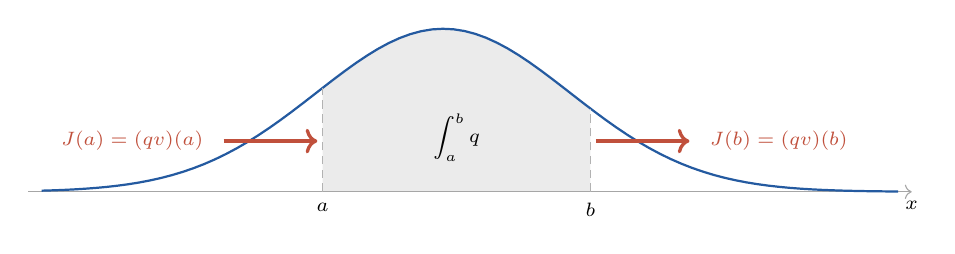
\begin{tikzpicture}[xscale=3.4, yscale=2.3]
\fill[gray!16] plot[domain=-0.45:0.55, samples=40]
  (\x, {0.9*exp(-\x*\x/0.45)}) -- (0.55, 0) -- (-0.45, 0) -- cycle;
\draw[->, gray!70] (-1.55,0) -- (1.75,0)
  node[below, font=\scriptsize, black] {$x$};
\draw[cdata, thick] plot[domain=-1.5:1.7, samples=80]
  (\x, {0.9*exp(-\x*\x/0.45)});
\draw[gray!60, densely dashed] (-0.45, 0)
  -- (-0.45, {0.9*exp(-0.2025/0.45)});
\draw[gray!60, densely dashed] (0.55, 0)
  -- (0.55, {0.9*exp(-0.3025/0.45)});
\node[below, font=\scriptsize] at (-0.45, -0.01) {$a$};
\node[below, font=\scriptsize] at (0.55, -0.01) {$b$};
\draw[->, cnoise, very thick] (-0.82, 0.28) -- (-0.47, 0.28);
\node[font=\scriptsize, cnoise, anchor=east] at (-0.86, 0.28)
  {$J(a) = (qv)(a)$};
\draw[->, cnoise, very thick] (0.57, 0.28) -- (0.92, 0.28);
\node[font=\scriptsize, cnoise, anchor=west] at (0.96, 0.28)
  {$J(b) = (qv)(b)$};
\node[font=\scriptsize] at (0.05, 0.30) {$\displaystyle\int_a^b q$};
\end{tikzpicture}
\caption{Probability is a conserved fluid: the mass in $[a, b]$ changes only by
the flux $J = qv$ through the endpoints --- in at $a$, out at $b$ ---
and shrinking the interval turns that sentence into
$\partial_t q + \partial_x(qv) = 0$. Every density-evolution equation in
these notes (continuity, Fokker--Planck, the probability-flow
rewriting) is this bookkeeping with a particular flux plugged in.}
\label{fig:flux}
\end{figure}

Two directions of travel through \eqref{eq:continuity}, and we use both.
\emph{Forward}: given the flow, the transported density satisfies
continuity --- that is the derivation above. \emph{Converse}, the
direction that does the real work later: \eqref{eq:continuity} is the
\emph{complete signature} of transport. If a family of densities $q_t$
and a velocity field $v_t$ satisfy \eqref{eq:continuity}, then sampling
$x_0 \sim q_0$ and integrating $\dot x = v_t(x)$ produces
$x_t \sim q_t$ at every time --- because (for fields as nice as ours)
the equation propagates $q_0$ forward uniquely, and the transported
density is one solution, hence the only one. Keep this converse loaded:
the central manoeuvre of Section~\ref{sec:pfode} will be to stare at a
PDE until it looks like \eqref{eq:continuity} for some velocity field,
and then to declare victory --- legitimately, because of exactly this
paragraph.

\subsection{How density changes along your own trajectory}
\label{sec:cov}

One more deterministic fact, three lines long, with an entire likelihood
theory hanging off it. Ride a particle: how does the density \emph{at
your own position} evolve? The $\tfrac{\dd}{\dd t}$ below is the
\emph{total} derivative along the moving particle --- both arguments of
$\log q_t(x_t)$ carry the $t$ --- which fluid mechanics calls the
material derivative $\partial_t + v \cdot \nabla$; the Eulerian
$\partial_t$ at a fixed point is only its first term. Chain rule plus
continuity:
\begin{equation}
\frac{\dd}{\dd t} \log q_t(x_t)
= \partial_t \log q_t + \dot x \cdot \nabla \log q_t
= \big( -\nabla\!\cdot\!v - v \cdot \nabla \log q_t \big)
+ v \cdot \nabla \log q_t ,
\end{equation}
expanding $\partial_t q = -\nabla\!\cdot\!(qv) = -q\,\nabla\!\cdot\!v
- v\!\cdot\!\nabla q$ and dividing by $q$. The advection terms cancel
and what survives is the \textbf{instantaneous change-of-variables
formula}
\begin{equation}
\boxed{\;\frac{\dd}{\dd t} \log q_t(x_t) = -\nabla\!\cdot\!v(x_t, t).\;}
\label{eq:cov}
\end{equation}
Read it physically: $\nabla\!\cdot\!v$ is the local rate of volume
expansion, and density dilutes exactly as fast as the volume around you
stretches --- conservation again, now per-particle. (It is also the
familiar change-of-variables Jacobian done infinitesimally:
$\log\det$ of the flow map's Jacobian grows at rate $\nabla\!\cdot\!v$.)
This formula is the entire likelihood machinery of continuous
normalizing flows, and Section~\ref{sec:likelihood} will cash it in for
diffusion models.

\begin{exercise}
\label{ex:cov-check}
Check \eqref{eq:cov} by hand for the scale flow $\dot x = c_t\, x$ in
$\R^d$ with $q_0 = \mathcal{N}(0, s^2 I)$: solve the flow, write down
$q_t$, and verify that both sides equal $-d\, c_t$ along every
trajectory.
\end{exercise}

\begin{recap}
A Lipschitz velocity field integrates to a flow: a composable family of
bijections whose trajectories never cross (uniqueness) and which
reverses by flipping a sign --- two free gifts the stochastic world will
conspicuously lack. A density carried by the flow obeys the continuity
equation $\partial_t q = -\nabla\!\cdot\!(qv)$, which is nothing but
``flux $=$ density $\times$ velocity'' plus conservation; conversely,
any $(q_t, v_t)$ pair satisfying it is realized by integrating the
field. Along your own trajectory, $\log q$ changes at rate
$-\nabla\!\cdot\!v$: density dilutes as volume stretches.
\end{recap}

\section{Interlude: the SDE toolkit, from a standing start}
\label{sec:sde}

The sampling sections ahead run on stochastic differential equations
and on their density-level shadows; this is the stochastic twin of the
toolkit just built, and it is genuinely small: one process (Brownian
motion), one rule (It\^o's lemma, which is Taylor's theorem plus a
single new fact), one solvable family (linear SDEs --- the only SDEs
this subject ever asks us to solve), and one bridge from paths to
densities (Fokker--Planck, which will turn out to be the continuity
equation with one extra flux). Readers who can solve an
Ornstein--Uhlenbeck equation without pausing should read the recap at
the end of the section and skip ahead.

\subsection{Brownian motion: $\sqrt{\dd t}$ is the whole personality}
\label{sec:bm}

A standard \textbf{Brownian motion} (or Wiener process) $W_t$ in $\R^d$
is the process with $W_0 = 0$, continuous paths, independent increments,
and
\begin{equation}
W_t - W_s \;\sim\; \mathcal{N}\big(0,\, (t-s)\, I\big),
\qquad 0 \le s < t.
\end{equation}
That such a process exists is a theorem (Wiener, 1923); we take it off
the shelf. Everything you need to know about it follows from one number:
over a window of length $\dd t$, the typical displacement is
$\sqrt{\dd t}$. Stare at that scaling --- $\sqrt{\dd t} \gg \dd t$ for
small $\dd t$ --- and two consequences fall out.

\emph{First: no velocity.} The difference quotient
$\Delta W / \Delta t \sim \Delta t^{-1/2}$ blows up as the window
shrinks: Brownian paths are continuous everywhere and differentiable
nowhere. A Brownian particle has a position at every time and a velocity
at none. (File this away: it is why the subject will have to work to
extract a \emph{deterministic} velocity field from a stochastic process,
an extraction Section~\ref{sec:pfode} supplies.)

\emph{Second: squared noise is not noise.} Take a partition
$0 = t_0 < \cdots < t_n = t$ with mesh $\max_k \Delta t_k \to 0$ and sum
the \emph{squared} increments of a scalar Brownian motion:
\begin{equation}
\sum_{k} \big( W_{t_{k+1}} - W_{t_k} \big)^2 \;\longrightarrow\; t
\qquad \text{in } L^2.
\label{eq:qv}
\end{equation}
The mean of the left side is $\sum_k \Delta t_k = t$ on the nose, and
its variance is $\sum_k 2\,\Delta t_k^2 \le 2t \max_k \Delta t_k \to 0$
(Exercise~\ref{ex:qv}). A sum of squared noises is deterministic: it is
elapsed time in disguise. This is the \textbf{quadratic variation} of
Brownian motion, and we abbreviate it as
\begin{equation}
(\dd W)^2 = \dd t, \qquad \dd t \cdot \dd W = o(\dd t), \qquad
(\dd t)^2 = o(\dd t).
\label{eq:dw2}
\end{equation}
Figure~\ref{fig:bm} shows both faces: paths that fill out a
$\sqrt{t}$ envelope while individually refusing to be smooth, and squared
increments whose running sum hugs the diagonal more tightly the finer
you chop.

\begin{exercise}
\label{ex:qv}
Prove \eqref{eq:qv}: using $\E[\xi^4] = 3$ for $\xi \sim \mathcal{N}(0,1)$,
show each squared increment has mean $\Delta t_k$ and variance
$2\Delta t_k^2$, and conclude by independence.
\end{exercise}

\begin{figure}[t]
\centering
\begin{tikzpicture}
\begin{axis}[
  dfm, width=7.6cm, height=5.6cm, axis lines=left,
  xmin=0, xmax=1, ymin=-2.4, ymax=2.4,
  xlabel={$t$}, ylabel={$W_t$},
  title={(a) three Brownian paths},
]
\addplot[gray, dashed, domain=0:1, samples=100] {2*sqrt(x)};
\addplot[gray, dashed, domain=0:1, samples=100] {-2*sqrt(x)};
\addplot[cdata, line width=0.5pt, unbounded coords=jump]
  table[x=t, y=w] {dfm_figs/bm_paths.dat};
\node[font=\scriptsize, gray, anchor=south] at (axis cs:0.78,1.78)
  {$\pm 2\sqrt{t}$};
\end{axis}
\end{tikzpicture}\hfill
\begin{tikzpicture}
\begin{axis}[
  dfm, width=7.6cm, height=5.6cm, axis lines=left,
  xmin=0, xmax=1, ymin=0, ymax=1.35,
  xlabel={$t$}, ylabel={$\sum (\Delta W)^2$},
  title={(b) quadratic variation: squared noise is time},
  legend pos=north west, legend cell align=left,
]
\addplot[gray, dashed, domain=0:1] {x};
\addlegendentry{$t$}
\addplot[cnoise, line width=0.6pt] table[x=t, y=qv] {dfm_figs/qv_16.dat};
\addlegendentry{$n = 16$}
\addplot[cflow, line width=0.6pt] table[x=t, y=qv] {dfm_figs/qv_256.dat};
\addlegendentry{$n = 256$}
\addplot[cdata, line width=0.6pt] table[x=t, y=qv] {dfm_figs/qv_4096.dat};
\addlegendentry{$n = 4096$}
\end{axis}
\end{tikzpicture}
\caption{The two faces of $\sqrt{\dd t}$. (a)~Sample Brownian paths:
individually rough beyond repair (zooming in never makes them look
smoother --- the wiggles are scale-free), collectively filling out the
$\pm 2\sqrt{t}$ envelope. (b)~The running sum of \emph{squared}
increments of one fixed path, chopped into $n$ pieces: as the mesh
refines, randomness drains out of the sum and it converges to the
diagonal --- equation \eqref{eq:qv}, $(\dd W)^2 = \dd t$, in pictures.}
\label{fig:bm}
\end{figure}

\subsection{What an SDE actually says}

The expression
\begin{equation}
\dd x = f(x, t)\, \dd t + g_t\, \dd W
\label{eq:sde-generic}
\end{equation}
is shorthand for an integral equation,
$x_t = x_0 + \int_0^t f(x_s, s)\,\dd s + \int_0^t g_s\, \dd W_s$, but for
our purposes the honest definition is operational: \eqref{eq:sde-generic}
is the small-$h$ limit of the simulation
\begin{equation}
x_{t+h} \;=\; x_t + f(x_t, t)\, h + g_t\, \sqrt{h}\; \xi_t,
\qquad \xi_t \sim \mathcal{N}(0, I) \text{ i.i.d.},
\label{eq:em}
\end{equation}
the \textbf{Euler--Maruyama} scheme --- drift times $h$, noise times
$\sqrt{h}$, with the $\sqrt{h}$ now unsurprising. For Lipschitz $f$ the
limit exists and is unique; ours will be \emph{linear} in $x$, the
friendliest possible case.\footnote{One genuine subtlety is dodged here:
if the noise amplitude depended on the state, $g(x_t, t)$, the limit of
\eqref{eq:em} would depend on \emph{where in the interval} you evaluate
$g$ --- evaluate at the left endpoint and you get the It\^o integral,
at the midpoint and you get Stratonovich, and the two differ by a drift
term of size $O(g\,\partial_x g)$, because $g$'s fluctuations correlate
with $\dd W$'s. Every SDE in the diffusion-model literature has
$g$ depending on $t$ only, so the ambiguity never bites, and we shall
not mention it again.}

\subsection{It\^o's lemma is Taylor's theorem with one extra term}

How does a smooth function $\varphi$ of the state evolve? Expand to
second order and keep everything of size $\dd t$:
\begin{equation}
\dd \varphi
= \nabla\varphi \cdot \dd x
+ \tfrac12\, \dd x^\top (\nabla^2 \varphi)\, \dd x + \cdots,
\qquad
\dd x\, \dd x^\top = \big(f \dd t + g\, \dd W\big)\big(\cdots\big)^\top
= g_t^2\, I\, \dd t + o(\dd t),
\end{equation}
using \eqref{eq:dw2} to kill every term except the $\dd W \dd W^\top$
square. The result is \textbf{It\^o's lemma}:
\begin{equation}
\boxed{\;\dd \varphi
= \Big( f \cdot \nabla\varphi
+ \tfrac{g_t^2}{2}\, \Delta\varphi \Big)\, \dd t
+ g_t\, \nabla\varphi \cdot \dd W.\;}
\label{eq:ito}
\end{equation}
The deterministic chain rule keeps only first-order terms; the
stochastic chain rule must keep the second-order one, because the square
of noise is time. That $\tfrac{g^2}{2}\Delta$ is the source of every
diffusion term in every PDE of this subject. Sanity check, $\varphi = x^2$
for pure Brownian motion ($f = 0$, $g = 1$, scalar):
$\dd(W^2) = \dd t + 2W\,\dd W$, so $\E[W_t^2] = t$ --- the variance
growth recovered as a calculus statement.

\begin{exercise}
Use \eqref{eq:ito} with $\varphi = x^4$ to show $\E[W_t^4] = 3t^2$,
confirming the fourth-moment input to Exercise~\ref{ex:qv}.
\end{exercise}

\subsection{Linear SDEs, solved completely --- and the forward SDE derived}
\label{sec:linsde}

Now the family we actually use:
$\dd x = f_t\, x\, \dd t + g_t\, \dd W$ with time-dependent scalars
$f_t, g_t$. Set $\alpha_t = \exp\big(\int_0^t f_s \dd s\big)$ and change
variables to $y = x / \alpha_t$. Because $\alpha_t$ is deterministic and
$y$ is linear in $x$ (so $\nabla^2 y = 0$ and It\^o's correction
vanishes), plain calculus applies:
\begin{equation}
\dd y = \frac{\dd x}{\alpha_t} - \frac{x\, \dot\alpha_t}{\alpha_t^2}\,\dd t
= \frac{g_t}{\alpha_t}\, \dd W
\quad\Longrightarrow\quad
x_t = \alpha_t\, x_0 + \alpha_t \int_0^t \frac{g_s}{\alpha_s}\, \dd W_s .
\label{eq:linsol}
\end{equation}
The integral is a weighted sum of independent Gaussian increments with
deterministic weights, hence Gaussian, with mean zero and variance given
by the \textbf{It\^o isometry}
$\E\big[\big(\int h_s \dd W_s\big)^2\big] = \int h_s^2\, \dd s$
(Exercise~\ref{ex:isometry}). Therefore
\begin{equation}
x_t \mid x_0 \;\sim\; \mathcal{N}\big( \alpha_t x_0,\; \sigma_t^2 I \big),
\qquad
\sigma_t^2 = \alpha_t^2 \int_0^t \frac{g_s^2}{\alpha_s^2}\, \dd s .
\label{eq:lingauss}
\end{equation}
This is exactly the interpolant \eqref{eq:interpolant}'s conditional law
--- and now run the logic \emph{backwards}. Given a designer pair
$(\alpha_t, \sigma_t)$, what SDE realizes it? Matching the mean forces
$f_t = \dot\alpha_t / \alpha_t$; differentiating the variance relation in
\eqref{eq:lingauss} gives
$\tfrac{\dd}{\dd t}\sigma_t^2 = 2 f_t \sigma_t^2 + g_t^2$, i.e.
\begin{equation}
g_t^2 = 2\sigma_t\dot\sigma_t - 2\,\frac{\dot\alpha_t}{\alpha_t}\,\sigma_t^2 .
\end{equation}
These are precisely the coefficients that will appear in
Section~\ref{sec:pfode}: not an ansatz to be checked but the unique
linear SDE with the prescribed conditional law.

The constant-coefficient case $f_t \equiv -\theta$, $g_t \equiv g$ is the
\textbf{Ornstein--Uhlenbeck process}: mean decays like $e^{-\theta t}$,
variance saturates at $g^2/2\theta$, and the process forgets its initial
condition exponentially fast, equilibrating to
$\mathcal{N}(0, \tfrac{g^2}{2\theta})$. The VP diffusion is an OU process
on a deformed clock --- which is the path-level picture of ``data is
shredded into a standard Gaussian.'' Figure~\ref{fig:ou} shows it
happening.

\begin{exercise}
\label{ex:isometry}
Prove the It\^o isometry for piecewise-constant $h$: expand the square
of $\sum_k h_{t_k} (W_{t_{k+1}} - W_{t_k})$ and use independence of
increments. (General $h$ follows by approximation; take that on faith.)
\end{exercise}

\begin{figure}[t]
\centering
\begin{tikzpicture}
\begin{axis}[
  dfm, width=12.6cm, height=6.2cm, axis lines=left,
  xmin=-0.02, xmax=1.16, ymin=-3.25, ymax=3.25,
  xlabel={$t$}, ylabel={$x$},
  xtick={0,0.25,0.5,0.75,1},
]
\addplot[fill=gray!13, draw=gray!40, very thin, forget plot]
  table[x=t, y=x] {dfm_figs/ou_env_0.dat};
\addplot[fill=gray!13, draw=gray!40, very thin, forget plot]
  table[x=t, y=x] {dfm_figs/ou_env_1.dat};
\addplot[fill=gray!14, draw=gray!50, very thin, forget plot]
  table[x=tt, y=x] {dfm_figs/prof3_4.dat};
\addplot[black!70, densely dashed, unbounded coords=jump, forget plot]
  table[x=t, y=x] {dfm_figs/ou_mean.dat};
\addplot[cnoise, line width=0.45pt, opacity=0.9, unbounded coords=jump,
  forget plot] table[x=t, y=x] {dfm_figs/ou_paths.dat};
\addplot[only marks, mark=*, mark size=1.4pt, black, forget plot]
  coordinates {(0,-1) (0,1)};
\node[font=\scriptsize, anchor=south] at (axis cs:0.5,2.62)
  {forward in time $\longrightarrow$ : data is shredded};
\node[font=\scriptsize, black!70, anchor=west] at (axis cs:0.30,1.06)
  {$\alpha_t x_0$};
\end{axis}
\end{tikzpicture}
\caption{The forward VP diffusion doing its one job, simulated by
Euler--Maruyama \eqref{eq:em} from the two data modes $x_0 = \pm 1$
(red paths). Dashed: the conditional means $\alpha_t x_0$ from
\eqref{eq:lingauss}, sliding to zero. Gray tubes: the conditional
$\pm 2\sigma_t$ bands, inflating until the two tubes merge; by $t = 1$
the marginal is the standard Gaussian (right profile), and nothing about
a path's endpoint betrays which mode it came from. Same picture as
Figure~\ref{fig:pfode}, opposite direction of travel: this is the easy
direction, and the entire subject is the art of traversing it backwards.}
\label{fig:ou}
\end{figure}

\subsection{From paths to densities: the Fokker--Planck equation}
\label{sec:fokker}

A process is a cloud of paths; call the cloud's density $q_t$.
Section~\ref{sec:continuity} taught us how to find a density's PDE:
identify the flux. The drift is a velocity field like any other and
contributes the advective flux $f(x, t)\, q_t$ of \eqref{eq:continuity}.
The genuinely new question is what flux the \emph{noise} carries.
Isolate it: take pure noise, $\dd x = g_t\, \dd W$. One step is a
Gaussian blur --- $x_{t+h} = x_t + g\sqrt{h}\,\xi$ convolves the density
with $\mathcal{N}(0, g^2 h I)$ --- so Taylor-expand under the
convolution:
\begin{equation}
q_{t+h}(x)
= \E_\xi\big[ q_t(x - g\sqrt{h}\,\xi) \big]
= q_t(x)
- g\sqrt{h}\;\underbrace{\E[\xi]}_{=\,0}\!\cdot\nabla q_t
+ \tfrac{g^2 h}{2}\,
\underbrace{\E\big[ \xi^\top (\nabla^2 q_t)\, \xi \big]}_{=\,\Delta q_t}
+ \;O(h^2),
\end{equation}
using $\E[\xi \xi^\top] = I$ and the vanishing of all odd moments. So
pure noise obeys $\partial_t q = \tfrac{g^2}{2} \Delta q$ --- the heat
equation --- and the heat equation is itself in conservation form:
$\tfrac{g^2}{2}\Delta q
= -\nabla\!\cdot\!\big( -\tfrac{g^2}{2} \nabla q \big)$. Diffusion is a
flux $-\tfrac{g^2}{2}\nabla q$ that drives probability \emph{down its
own density gradient} --- Fick's law, here derived rather than
postulated. Drift and noise contribute independently at order $h$
(their cross-terms are $O(h^{3/2})$), so the fluxes add:
\begin{equation}
\boxed{\;\partial_t q_t
= -\nabla\!\cdot\!\big( f\, q_t \big)
+ \tfrac{g_t^2}{2}\, \Delta q_t
\;=\; -\nabla\!\cdot\!\Big( \underbrace{f\, q_t
- \tfrac{g_t^2}{2}\, \nabla q_t}_{\text{total flux}} \Big).\;}
\label{eq:fp-general}
\end{equation}
This is \textbf{Fokker--Planck} (the physicists' name) or
\textbf{Kolmogorov forward} (the probabilists'): the continuity
equation with the flux enlarged from $qv$ to advection plus
down-gradient diffusion --- probability still neither created nor
destroyed, only carried and spread. And --- this is the loaded gun
placed on the mantelpiece --- the equation depends on the process only
through the pair $(f, g_t^2)$ \emph{and constrains only the marginals}:
very different processes can share one and the same family $q_t$.
Section~\ref{sec:pfode} fires this gun.

\begin{exercise}
Re-derive \eqref{eq:fp-general} the weak way: take expectations of
It\^o's lemma \eqref{eq:ito} (the $\dd W$ term has mean zero and dies),
write $\tfrac{\dd}{\dd t}\E[\varphi(x_t)]
= \E[f \cdot \nabla\varphi + \tfrac{g^2}{2}\Delta\varphi]$ as integrals
against $q_t$, and integrate by parts --- once on the drift term, twice
on the diffusion term --- to move the derivatives onto the density.
Same equation, different dress.
\end{exercise}

\subsection{Langevin dynamics: the SDE that stands still}
\label{sec:langevin}

One special case deserves its own subsection. Fix a target density $p$
and consider, for a step-size parameter $\eta > 0$,
\begin{equation}
\dd x = \tfrac{\eta}{2}\, \nabla \log p(x)\, \dd t + \sqrt{\eta}\, \dd W .
\label{eq:langevin}
\end{equation}
Plug $f = \tfrac{\eta}{2}\nabla\log p$, $g^2 = \eta$ into
\eqref{eq:fp-general} and evaluate at $q = p$:
\begin{equation}
-\tfrac{\eta}{2} \nabla\!\cdot\!\big( p\, \nabla\log p \big)
+ \tfrac{\eta}{2}\, \Delta p
= -\tfrac{\eta}{2} \nabla\!\cdot\!\big( \nabla p \big)
+ \tfrac{\eta}{2}\, \Delta p = 0 ,
\end{equation}
using $p\,\nabla\log p = \nabla p$. So $p$ is stationary: the
score-driven drift uphill exactly balances the diffusive spreading.
\textbf{Langevin dynamics} is the SDE that goes nowhere, distributionally
--- and notice what it needs: \emph{only the score}, the
normalization-free object of Section~\ref{sec:score}. Run
\eqref{eq:langevin} long enough and (under conditions we will not fuss
over) it samples $p$. Why is that not already a generative model, given a
learned score at noise level zero? Because Langevin mixes between
well-separated modes at a rate that is exponentially small in the barrier
height, and near a low-dimensional data manifold the score is enormous
and ill-behaved off-manifold. The historical fix (annealed Langevin,
SMLD) and the modern subject are the same idea: maintain the whole family
$\{q_t\}$, mix at high noise where mixing is free, and use the
low-noise scores only for the final approach. Keep \eqref{eq:langevin}
in your pocket: in Section~\ref{sec:pfode} it reappears inside the
reverse-time SDE as the ``churn'' that holds a sampler on the marginal
$q_t$ while transport does the real work.

\begin{exercise}
\label{ex:divfree}
Show that adding any vector field $u$ with
$\nabla\!\cdot\!(p\, u) = 0$ to the drift of \eqref{eq:langevin} leaves
$p$ stationary. (Moral: the dynamics realizing given marginals are never
unique --- remember this when the marginal velocity of
Section~\ref{sec:fm} is introduced with a definite article.)
\end{exercise}

\begin{recap}
Brownian increments scale as $\sqrt{\dd t}$, so squared increments are
deterministic: $(\dd W)^2 = \dd t$. That single fact upgrades Taylor to
It\^o \eqref{eq:ito}, solves every linear SDE in closed form ---
yielding exactly the interpolant's Gaussian conditionals and hence,
read backwards, deriving the forward SDE's coefficients --- and, in
expectation, turns path statements into the density statement
\eqref{eq:fp-general}. Langevin dynamics is the special SDE whose
Fokker--Planck flow vanishes: score drift balancing diffusion, the
score's normalization-freeness made kinetic.
\end{recap}

\section{Sampling I: the probability flow ODE}
\label{sec:pfode}

We have (an estimate of) the scores. How do they generate? The cleanest
route --- cleaner than the historical one --- goes through a small
calculation with the Fokker--Planck equation \eqref{eq:fp-general}, and
it is worth doing in full because it is three lines and it manufactures
the bridge between diffusions and flows.

The interpolant \eqref{eq:interpolant} can be realized as a forward-time
SDE that gradually shreds data,
\begin{equation}
\dd x = f_t\, x\, \dd t + g_t\, \dd W, \qquad
f_t = \frac{\dot\alpha_t}{\alpha_t}, \quad
g_t^2 = 2\big(\sigma_t\dot\sigma_t - \sigma_t^2 \tfrac{\dot\alpha_t}{\alpha_t}\big),
\label{eq:forward-sde}
\end{equation}
--- these coefficients were \emph{derived} in Section~\ref{sec:linsde}:
match the conditional mean to get $f_t$, differentiate the conditional
variance to get $g_t$. (Note also
$g_t^2 = 2\sigma_t^2 \tfrac{\dd}{\dd t}\log(\sigma_t/\alpha_t)$, which is
nonnegative precisely when the signal-to-noise ratio
$\alpha_t^2/\sigma_t^2$ is decreasing --- a schedule is realizable as a
diffusion exactly when it destroys information at every instant.) Its
marginals obey Fokker--Planck \eqref{eq:fp-general} with linear drift:
\begin{equation}
\partial_t q_t = -\nabla\!\cdot\!\big( f_t\, x\, q_t \big)
+ \tfrac{g_t^2}{2}\, \Delta q_t .
\end{equation}
Now the move. The diffusion term is also a divergence --- of a flux
proportional to the score:
$\Delta q_t = \nabla\!\cdot\!\nabla q_t
= \nabla\!\cdot\!\big( q_t\, \nabla\log q_t \big)$. Substitute and gather:
\begin{equation}
\partial_t q_t
= -\nabla\!\cdot\!\Big[ \Big( \underbrace{f_t\, x
- \tfrac{g_t^2}{2}\, \nabla\log q_t(x)}_{\textstyle v_t(x)} \Big)\, q_t \Big].
\label{eq:pf}
\end{equation}
But \eqref{eq:pf} is precisely the continuity equation
\eqref{eq:continuity} for the velocity field $v_t$ --- and the converse
direction of Section~\ref{sec:continuity} now does the work: the same
family of marginals $q_t$ is carried by the deterministic ODE
$\dot x = v_t(x)$. No noise anywhere. The stochastic shredding process and
this \textbf{probability flow ODE} are statistically indistinguishable at
the level of single-time marginals --- and the ODE can be run
\emph{backwards}, from $x_1 \sim \mathcal{N}(0, I)$ to a data sample, by
any off-the-shelf integrator, with the learned score plugged in
(Section~\ref{sec:solvers} examines how few steps the integrator can get
away with).

\emph{The randomness of the diffusion was an
implementation detail.} The footprint it leaves on the marginals can be
reproduced by a velocity field, and the velocity field is an affine
function of the score \eqref{eq:wardrobes}. Deterministic samplers (DDIM
is a particular discretization of this ODE), flow likelihoods (the
change-of-variables formula \eqref{eq:cov} applies the moment a flow
exists), and the entire flow-matching
viewpoint all enter through equation \eqref{eq:pf}.

And since the training loop got its six lines, generation deserves its
six --- the probability-flow ODE under Euler, run from noise back to
data:
\begin{lstlisting}
@torch.no_grad()
def sample_pf_ode_eps_model(model, shape, steps):
    x  = torch.randn(shape)                    # x_1 ~ N(0, I)
    n  = shape[0]
    bshape = (-1,) + (1,) * (x.ndim - 1)
    ts = torch.linspace(1.0, 0.0, steps + 1)
    for t, t_next in zip(ts[:-1], ts[1:]):
        tt = t.expand(n).to(x.device)
        score = -model(x, tt) / sigma(tt).view(bshape)  # epsilon -> score
        v = (f(tt).view(bshape) * x
             - 0.5 * g2(tt).view(bshape) * score)
        x = x + (t_next - t) * v                    # Euler, backwards
    return x
\end{lstlisting}
Swapping in the reverse SDE \eqref{eq:reverse-sde} adds one line of
injected noise; choosing the integrator, the step count, and where the
steps go is Section~\ref{sec:solvers}'s entire business.

\subsection{Sampling II: putting the noise back (and why you might)}

You can also reverse the SDE itself --- though, unlike the ODE, not for
free: Section~\ref{sec:odeflows}'s sign-flip gift is exclusive to
deterministic flows, because a Brownian increment does not unhappen when
you negate a drift. Reversal here costs a theorem and a score. The
classical result (Anderson, 1982)
is that the time-reversal of \eqref{eq:forward-sde} is again an SDE,
\begin{equation}
\dd x = \big[ f_t\, x - g_t^2\, \nabla\log q_t(x) \big]\, \dd t
+ g_t\, \dd \bar W \qquad (\text{run backwards}),
\label{eq:reverse-sde}
\end{equation}
with \emph{twice} the score correction of the ODE plus reinjected noise.
Anderson's theorem has a fearsome reputation and a four-line
proof-by-Bayes,\footnote{One Euler--Maruyama step of the forward SDE is
a Gaussian kernel $q(x_{t+h} \mid x_t)$. Bayes inverts it:
$q(x_t \mid x_{t+h}) \propto q(x_{t+h} \mid x_t)\, q_t(x_t)$. Expand
$\log q_t(x_t)$ to first order around $x_{t+h}$ and complete the square,
and out falls a Gaussian reverse kernel with mean
$x_{t+h} - h\big[ f_t\, x_{t+h} - g_t^2 \nabla\log q_t(x_{t+h}) \big] + O(h^2)$ and
covariance $g_t^2 h\, I$ --- one Euler--Maruyama step of
\eqref{eq:reverse-sde}. Problem~\ref{prob:anderson} asks you to push the
algebra through and locate where the factor of \emph{two}, relative to
the ODE's $\tfrac{g^2}{2}$, comes from.} so rather than dwell on the
proof, see the structure: \eqref{eq:reverse-sde}
$=$ probability-flow ODE $+$ $\big[\tfrac{g^2}{2}\nabla\log q_t\,\dd t +
g\,\dd\bar W\big]$, and that bracketed extra, per unit of \emph{reverse}
time, is precisely a step of
\emph{Langevin dynamics} \eqref{eq:langevin} targeting $q_t$ --- the SDE
that stands still (Section~\ref{sec:langevin}), leaving each marginal
invariant. So the reverse SDE is ``transport $+$ equilibration'':
the ODE part moves mass between noise levels; the Langevin part churns
within a noise level, correcting accumulated error at the cost of extra
stochasticity. Every sampler in the literature --- DDPM ancestral
sampling, DDIM with its $\eta$ knob, predictor--corrector schemes, EDM's
churn parameter --- is a point on this one-parameter family between pure
ODE and heavily-churned SDE. Deterministic is fast and reproducible;
stochastic forgives a sloppy score model.
Figure~\ref{fig:pfode} shows both samplers riding the same path of
marginals.

\begin{figure}[t]
\centering
\begin{tikzpicture}
\begin{axis}[
  dfm, width=13.4cm, height=7.0cm, axis lines=left,
  xmin=-0.02, xmax=1.16, ymin=-3.25, ymax=3.25,
  xlabel={$t$}, ylabel={$x$},
  xtick={0,0.25,0.5,0.75,1},
  legend pos=north west, legend cell align=left,
]
% marginal density profiles q_t at five times (normalized widths);
% forget plot keeps them out of the legend
\addplot[fill=gray!14, draw=gray!50, very thin, forget plot] table[x=tt, y=x] {dfm_figs/prof3_0.dat};
\addplot[fill=gray!14, draw=gray!50, very thin, forget plot] table[x=tt, y=x] {dfm_figs/prof3_1.dat};
\addplot[fill=gray!14, draw=gray!50, very thin, forget plot] table[x=tt, y=x] {dfm_figs/prof3_2.dat};
\addplot[fill=gray!14, draw=gray!50, very thin, forget plot] table[x=tt, y=x] {dfm_figs/prof3_3.dat};
\addplot[fill=gray!14, draw=gray!50, very thin, forget plot] table[x=tt, y=x] {dfm_figs/prof3_4.dat};
% one reverse-SDE path (drawn under the ODE bundle)
\addplot[cnoise, line width=0.55pt, opacity=0.85, unbounded coords=jump]
  table[x=t, y=x] {dfm_figs/sde3.dat};
\addlegendentry{reverse SDE \eqref{eq:reverse-sde}}
% probability-flow ODE trajectories
\addplot[cdata, line width=0.6pt, unbounded coords=jump]
  table[x=t, y=x] {dfm_figs/ode3.dat};
\addlegendentry{PF-ODE \eqref{eq:pf}}
% data modes
\addplot[only marks, mark=*, mark size=1.4pt, black] coordinates {(0,-1) (0,1)};
\node[font=\scriptsize, anchor=south] at (axis cs:0.62,2.62)
  {$\longleftarrow$ generation runs right to left};
\end{axis}
\end{tikzpicture}
\caption{One path of marginals, two ways to traverse it, computed exactly
for $p_{\mathrm{data}} = \tfrac12\mathcal{N}(-1, 0.1^2) +
\tfrac12\mathcal{N}(+1, 0.1^2)$ under the VP schedule
($\beta$ linear in $[0.1, 20]$). Gray profiles: the marginal density
$q_t$ at $t = 0, 0.25, \ldots, 1$ (widths normalized per slice), morphing
from two sharp data modes to a standard Gaussian. Blue: probability-flow
ODE trajectories \eqref{eq:pf} started from twelve quantiles of
$\mathcal{N}(0,1)$ and integrated backwards --- smooth, deterministic,
never crossing (the uniqueness gift of Section~\ref{sec:odeflows}),
splitting at the ridge between basins. Red: one
reverse-SDE path \eqref{eq:reverse-sde} from $x_1 = 0.1$ --- same drift
family, but the Langevin churn keeps it rattling around inside each
marginal before it commits to a mode. Both end with the correct
statistics; only the red one can change its mind.}
\label{fig:pfode}
\end{figure}

\begin{recap}
Rewriting the diffusion's Fokker--Planck equation as a continuity equation
shows its marginals are equally generated by a deterministic velocity
field $v_t = f_t x - \tfrac{g_t^2}{2}\nabla\log q_t$: the probability flow
ODE. The reverse SDE is this ODE plus marginal-preserving Langevin churn.
Sampling is numerical integration; the stochastic/deterministic choice is
a robustness/speed dial, not a modeling commitment.
\end{recap}

\section{Interlude: DDPM in discrete time --- the chain, the ELBO, the VAE}
\label{sec:elbo}

Before flows, two reconciliations with the literature's native dialect:
the discrete Markov chain that DDPM actually defines (and the
$\bar\alpha$ notation it spawned, a reliable generator of bugs), and the
ELBO that trains it --- which will turn out to be a VAE with every
classic failure mode engineered away.

\subsection{The discrete chain, and where $\bar\alpha$ comes from}
\label{sec:discrete}

DDPM as published is not an SDE; it is a Markov chain of $N$ corruption
steps,
\begin{equation}
q(x_k \mid x_{k-1})
= \mathcal{N}\big( \sqrt{1 - \beta_k}\; x_{k-1},\; \beta_k I \big),
\qquad k = 1, \ldots, N,
\label{eq:ddpm-chain}
\end{equation}
with small per-step variances $\beta_k$. The $\sqrt{1 - \beta_k}$ is the
variance-preserving choice in discrete dress: if
$\E\|x_{k-1}\|^2 = d$ then
$\E\|x_k\|^2 = (1 - \beta_k)\, d + \beta_k\, d = d$. Because each step is
a linear-Gaussian map, the chain composes in closed form (check by
adding variances of independent Gaussians):
\begin{equation}
x_k = \sqrt{\bar\alpha_k}\; x_0 + \sqrt{1 - \bar\alpha_k}\;\veps,
\qquad
\bar\alpha_k = \prod_{j \le k} (1 - \beta_j),
\qquad \veps \sim \mathcal{N}(0, I).
\label{eq:ddpm-marginal}
\end{equation}
Set this against the interpolant \eqref{eq:interpolant} and the
dictionary is
\begin{equation}
\alpha_{t_k} = \sqrt{\bar\alpha_k}, \qquad
\sigma_{t_k} = \sqrt{1 - \bar\alpha_k}
\qquad \text{--- \emph{DDPM's $\bar\alpha$ is our $\alpha$ squared}.}
\end{equation}
That single squaring is responsible for a measurable fraction of all
sign and scale errors in this literature (an early draft of
Figure~\ref{fig:schedules}'s caption included --- the author confidently
quoted an $\bar\alpha$ as an $\alpha$); when opening any paper, the
first thing to establish is whether its alphas are ours or their
squares.

The continuum limit connects the chain to everything we have built. Put
$\beta_k = \beta(t_k)\, h$ with $h = 1/N$ and expand
\eqref{eq:ddpm-chain}:
$\sqrt{1 - \beta h} = 1 - \tfrac12 \beta h + O(h^2)$, so one step reads
\begin{equation}
x_k - x_{k-1}
= -\tfrac12\, \beta(t_k)\, h\, x_{k-1} + \sqrt{\beta(t_k)\, h}\;\xi_k ,
\end{equation}
which is exactly one Euler--Maruyama step \eqref{eq:em} of the VP
forward SDE $\dd x = -\tfrac12 \beta x\, \dd t + \sqrt{\beta}\, \dd W$.
Likewise $\log \bar\alpha(t) = \sum_{j} \log(1 - \beta_j h)
\to -\int_0^t \beta$, recovering the table row of Section~1.1,
$\alpha_t = e^{-\frac12 \int_0^t \beta}$. The same correspondence runs
through sampling: DDPM's ancestral sampler is the Euler--Maruyama
discretization of the reverse SDE \eqref{eq:reverse-sde} (and
Problem~\ref{prob:anderson}'s Bayes-expansion derivation of Anderson is
nothing but this discrete chain inverted step by step, then sent to the
limit). Discrete DDPM and the continuous-time story are one model at two
resolutions; these notes stay continuous because the calculus is
lighter, and translate at the boundary with the dictionary above.

\subsection{The ELBO: a VAE with an incorruptible encoder}

Keep the discretization,
$0 = t_0 < t_1 < \cdots < t_N = 1$, and view
$x_{t_1}, \ldots, x_{t_N}$ as a \emph{hierarchy of latent variables} above
the data $x_0$. The forward corruption $q(x_{t_{k}} \mid x_{t_{k-1}})$ is
the encoder; the learned reverse model
$p_\theta(x_{t_{k-1}} \mid x_{t_k})$ is the decoder; the standard ELBO
telescopes into
\begin{equation}
\begin{aligned}
\log p_\theta(x_0) \;\geq\;&
\E_q\Big[ \log p_\theta(x_0 \mid x_{t_1}) \Big]
- \sum_{k=2}^{N}
\E_q\, \mathrm{KL}\Big(
q(x_{t_{k-1}} \mid x_{t_k}, x_0)
\,\big\|\, p_\theta(x_{t_{k-1}} \mid x_{t_k}) \Big)
\\
&- \mathrm{KL}\big( q(x_{t_N} \mid x_0) \,\|\, p(x_{t_N}) \big).
\end{aligned}
\label{eq:elbo}
\end{equation}
Read the three pieces from right to left. The final KL asks whether the
last corrupted sample is actually close to the chosen prior; it contains
no parameters, and with a long enough schedule it is also near zero. The middle sum is the real
training signal: at each noise level, the model's one-step reverse
Gaussian must match the analytic posterior one would get if the clean
$x_0$ were known. The first term is the final reconstruction or decoder
term at the data end, whose exact treatment depends on the data
likelihood convention (Gaussian for continuous data, discretized
logistic or categorical variants for pixels), but which plays the same
role as the bottom decoder term of an ordinary VAE.

Every middle term is between Gaussians. The forward posterior
$q(x_{t_{k-1}} \mid x_{t_k}, x_0)$ is Gaussian with closed-form mean
(Problem~\ref{prob:posterior}); if the reverse model uses the same
variance, its KL is just a constant times the squared error between the
true posterior mean and the model's predicted mean. Parameterize that
predicted mean by $\hat\veps_\theta$ using
\eqref{eq:ddpm-marginal}, and the same KL becomes a weighted version of
the noise-prediction loss \eqref{eq:dsm}. DDPM's celebrated ``simple
loss'' is \eqref{eq:elbo} with the per-level weights thrown away (which
empirically helps samples and hurts likelihoods --- you are reweighting
how much the model cares about coarse versus fine scales).

Now compare with the VAEs of your past life, because every classic failure
mode is structurally absent:
\begin{itemize}
\item The encoder is \emph{fixed and analytic} --- there is nothing to
collapse, no posterior to fight the prior, no pressure toward the mean
image. The eternal tug-of-war between reconstruction and KL has been
settled by fiat: the ``inference network'' is a noise schedule.
\item The latent has the data's dimension and the prior is exactly reached
by construction ($q_{t_N} \approx \mathcal{N}$): the aggregate-posterior
/ prior mismatch --- the hole-in-the-prior problem --- is engineered away.
\item What is given up: a one-shot encoder--decoder pass becomes an
$N$-step decoder, and the rich learned latent semantics of a good VAE are
replaced by~\dots\ noise. Diffusion buys its stability by making the latent
space maximally boring.\footnote{Latent diffusion gets some semantics back
by running the diffusion inside a (frozen) VAE's latent space --- the two
technologies composed, each doing what it is good at: the VAE compresses,
the diffusion generates.}
\end{itemize}

\section{Flow matching: regress on the velocity directly}
\label{sec:fm}

Section~\ref{sec:pfode} produced a velocity field by way of scores and
Fokker--Planck. Flow matching asks the impertinent question: \emph{why
take the detour?} If generation is just integrating $\dot x = v_t(x)$,
let's learn $v_t$ by regression, directly.

Two obstacles, both instructive. First, which $v_t$? For a given path of
marginals $\{q_t\}$ there are many velocity fields satisfying the
continuity equation (add any divergence-free-relative-to-$q_t$ field ---
this is Exercise~\ref{ex:divfree} again, minus the noise);
we should pick a canonical one. Second --- the apparent killer --- the
canonical choice depends on the unknown marginals, exactly as the score
did. The resolution is exactly the resolution of Section~\ref{sec:score},
which is the punchline of these notes: \emph{flow matching is
Lemma~\ref{lem:proj} applied to velocities instead of scores}.

\paragraph{Dictionary before the switch.}
Four vector fields are now in play, and keeping them separate prevents
most mistakes. The \textbf{score} $\score=\nabla\log q_t$ points up the
noisy marginal density. The \textbf{probability-flow velocity}
$f_t x-\tfrac12 g_t^2\score$ is the deterministic field manufactured
from that score in Section~\ref{sec:pfode}. The \textbf{conditional
velocity} below is a per-sample derivative of one interpolant path. The
\textbf{marginal velocity} is the posterior average of those conditional
velocities over all sample pairs passing through the same $x_t$; for the
Gaussian interpolants used in these notes, it will equal the
probability-flow velocity exactly.

Differentiate the interpolant \eqref{eq:interpolant} along its own clock:
each pair $(x_0, \veps)$ traces the \textbf{conditional path}
$x_t = \alpha_t x_0 + \sigma_t \veps$ with \textbf{conditional velocity}
\begin{equation}
\dot x_t = \dot\alpha_t\, x_0 + \dot\sigma_t\, \veps
\qquad \text{--- known, per sample, in closed form.}
\label{eq:cond-vel}
\end{equation}
Define the \textbf{marginal velocity} as the conditional average of
\eqref{eq:cond-vel} over everything passing through $x$ at time $t$:
\begin{equation}
v_t(x) \;=\; \E_{(x_0, \veps) \sim p(x_0, \veps \mid x_t = x)}
\big[ \dot\alpha_t x_0 + \dot\sigma_t \veps \big],
\label{eq:marg-vel}
\end{equation}
the measure spelled out as in \eqref{eq:dsm-identity}: the joint
posterior over \emph{pairs}, which is supported on the affine slice
$\{(x_0, \veps) : \alpha_t x_0 + \sigma_t \veps = x\}$ --- the phrase
``everything passing through $x$'' made into a probability
distribution, each line through $x$ weighted by how likely it was to be
the one you are on.
A short continuity-equation computation (Problem~\ref{prob:continuity})
confirms that \eqref{eq:marg-vel} transports the marginals $q_t$ ---
indeed, applying Tweedie \eqref{eq:tweedie} inside \eqref{eq:marg-vel}
reproduces \emph{exactly} the probability-flow velocity of \eqref{eq:pf}.
Same object, second derivation, no Fokker--Planck required.

And now Lemma~\ref{lem:proj}, verbatim, with
$A = \dot\alpha_t x_0 + \dot\sigma_t\veps$ and $B = (x_t, t)$: the
\textbf{conditional flow matching} objective
\begin{equation}
\boxed{\;\mathcal{L}_{\mathrm{CFM}}
= \E_{t,\,x_0,\,\veps}
\big\| v_\theta(x_t, t) - \big(\dot\alpha_t\, x_0 + \dot\sigma_t\, \veps\big) \big\|^2\;}
\label{eq:cfm}
\end{equation}
is minimized exactly at the marginal velocity \eqref{eq:marg-vel}, even
though the network only ever sees the crude per-sample targets
\eqref{eq:cond-vel}. The gradients of \eqref{eq:cfm} and of the intractable
``regress on $v_t$ directly'' objective coincide. (Figure~\ref{fig:lemma}
is once more the picture, with $\dot\alpha_t x_0 + \dot\sigma_t \veps$ in
place of $\veps$ on the vertical axis.)

Two remarks to let this land. First, put \eqref{eq:dsm} and \eqref{eq:cfm}
side by side: for this Gaussian-interpolant setting, they have the same
shape --- sample a pair, form the interpolant, regress on a closed-form
per-sample vector --- differing only in which member of the wardrobe
\eqref{eq:wardrobes} is worn. In that precise sense, score matching and
flow matching are two parameterizations of the same marginal transport
field. In the wider flow-matching literature one can choose more general
conditional paths and couplings, so the slogan should not be read as a
theorem about every object bearing the name. Second, the historical
significance for the flows community: continuous normalizing flows were
always elegant and always untrainable at scale, because computing the
likelihood meant \emph{solving the ODE inside the training loop}. Flow
matching is CNF training gone \emph{simulation-free}: no solver until
sampling time. That single property is why the method took over.

\subsection{Rectified flow: the case for straight lines}

Among schedules, the linear one --- $\alpha_t = 1 - t$, $\sigma_t = t$ ---
has a distinguished personality. Its conditional velocity
\eqref{eq:cond-vel} is \emph{constant in time}:
\begin{equation}
\dot x_t = \veps - x_0,
\end{equation}
each training pair contributing a straight line from data to noise
traversed at uniform speed, and the CFM target losing its time dependence
entirely: predict the displacement. (In the popular convention this is
``rectified flow'' or the ``stochastic interpolant'' with linear path;
it is the training objective behind several current large image models.)

Why care about straightness? Because of the cost model of sampling. The
expensive primitive is a network evaluation; an ODE whose trajectories are
straight is integrated \emph{exactly by one Euler step} (a slogan that
Section~\ref{sec:solvers} sharpens into a statement about truncation
error). Now, a subtlety
that is worth being slow about, because it is the most commonly garbled
point in the subject: \textbf{straight conditional paths do not make the
marginal ODE's trajectories straight}. The marginal velocity
\eqref{eq:marg-vel} is an \emph{average} of crossing straight lines, and
averaging straight lines that cross produces curved integral curves
(the average direction changes as the mix of lines overhead changes). The
linear schedule gives you straight \emph{targets} and a clean objective,
not one-step sampling. Figure~\ref{fig:reflow} shows the distinction at a
glance, and the resolution. The genuinely clever move --- \emph{reflow}
(rectification) --- is iterative: sample pairs $(x_1, x_0')$ by running
your current model's ODE, so that endpoints are \emph{coupled} rather than
independent, and retrain on the linear interpolant of these non-crossing
pairs. Each round provably straightens trajectories (it can only reduce
the transport cost), and a round or two gets close enough to straight that
one--four step sampling works. Distillation methods (consistency models,
progressive distillation) attack the same step-count problem by other
means; the underlying currency is always trajectory curvature versus
network calls.\footnote{Readers of the previous notes in this series will
recognize the shape of the argument: the cost model (network evaluations)
selects the geometry (straight paths) --- choose the chart in which your
expensive primitive is cheap. Table-making lessons transfer.}

\begin{figure}[t]
\centering
\begin{tikzpicture}
\begin{axis}[
  dfm, width=7.6cm, height=6.4cm, axis lines=left,
  xmin=-0.02, xmax=1.02, ymin=-2.7, ymax=2.7,
  xlabel={$t$}, ylabel={$x$}, xtick={0,0.5,1},
  title={(a) independent coupling},
]
\addplot[gray!65, line width=0.5pt, unbounded coords=jump]
  table[x=t, y=x] {dfm_figs/lines4.dat};
\addplot[cdata, line width=0.7pt, unbounded coords=jump]
  table[x=t, y=x] {dfm_figs/ode4.dat};
\addplot[only marks, mark=*, mark size=1.6pt, black] coordinates {(0,-1) (0,1)};
\end{axis}
\end{tikzpicture}\hfill
\begin{tikzpicture}
\begin{axis}[
  dfm, width=7.6cm, height=6.4cm, axis lines=left,
  xmin=-0.02, xmax=1.02, ymin=-2.7, ymax=2.7,
  xlabel={$t$}, xtick={0,0.5,1}, ytick=\empty,
  title={(b) reflow coupling},
]
\addplot[cflow, line width=0.7pt, unbounded coords=jump]
  table[x=t, y=x] {dfm_figs/reflow4.dat};
\addplot[only marks, mark=*, mark size=1.6pt, black] coordinates {(0,-1) (0,1)};
\end{axis}
\end{tikzpicture}
\caption{Straight targets versus straight trajectories, exactly computed
for data concentrated at $x_0 = \pm 1$ with the linear schedule. (a)~Under
the independent coupling of training, the conditional paths (gray) are
straight lines from each data point to each noise sample --- and they
cross. The marginal velocity \eqref{eq:marg-vel} at a crossing point must
average the gray directions overhead, so the integral curves of the
probability-flow ODE (blue) bend: flat near $t = 1$ where the average is
dominated by ``head for the origin,'' then committing to a mode as the
posterior sharpens. Euler with one step would follow the tangent at
$t = 1$ and miss. (b)~Reflow replaces the coupling: each noise point is
paired with \emph{its own ODE endpoint}, and the straight interpolants of
these coupled pairs (teal) no longer cross (non-crossing again: the
uniqueness gift of Section~\ref{sec:odeflows} makes the one-dimensional
flow monotone, so the coupling is order-preserving). Retrained on these
pairs, the marginal flow has straight
trajectories and one Euler step is exact. The coupling change, not the
linear schedule, is the active ingredient.}
\label{fig:reflow}
\end{figure}

\subsection{The optimal transport vista}
\label{sec:ot}

The abstract promised a community that ``speaks of optimal transport,''
and one debt from the toolkit is still outstanding:
Exercise~\ref{ex:divfree} showed that the dynamics realizing a given
family of marginals are never unique, and left hanging the question
\emph{then which one?} Optimal transport is the principled answer, and
--- now that the continuity equation is built --- it costs one
definition. The \textbf{Benamou--Brenier} formulation: among all pairs
$(q_t, v_t)$ satisfying the continuity equation \eqref{eq:continuity}
with prescribed endpoints $q_0$ and $q_1$, choose the one of least total
kinetic energy,
\begin{equation}
\inf_{(q, v)}\; \int_0^1 \!\!\int \big\| v_t(x) \big\|^2\, q_t(x)\,
\dd x\, \dd t
\qquad \text{subject to} \qquad
\partial_t q + \nabla\!\cdot\!(q v) = 0,\quad
q_0, q_1 \text{ fixed.}
\label{eq:bb}
\end{equation}
The character of the minimizer is the one sentence we actually need:
\emph{every particle travels in a straight line at constant speed}, and
the optimal value is (by definition, if you like) the squared
Wasserstein-2 distance $W_2^2(q_0, q_1)$ --- we need the phrase, not the
theory. Why straight lines? The population problem inherits a
single-particle fact: for a path $\gamma$ on $[0,1]$ with fixed
endpoints, $\int_0^1 \|\dot\gamma\|^2\, \dd t \ge
\|\gamma(1) - \gamma(0)\|^2$, with equality exactly for constant
velocity (Exercise~\ref{ex:kinetic}) --- wiggling and speed variation
are pure energetic waste. On top of that, the optimal \emph{pairing} of
sources to targets never lets two transport rays cross: if they crossed,
swapping targets would lower the combined cost (one leg may lengthen;
for quadratic cost the sum cannot fail to drop). The same non-crossing
geometry, a third time.

Now place the subject on this map, honestly. \emph{One}: the
diffusion/flow-matching path of marginals is \textbf{not} the OT
geodesic. The Gaussian-corruption path was chosen for trainability ---
closed-form conditionals, Lemma~\ref{lem:proj} applicable --- not for
kinetic economy; the probability-flow field is the canonical transport
of a deliberately non-optimal path. \emph{Two}: rectified flow's
training pairs are straight rays with the \emph{independent} coupling,
and independent rays cross (Figure~\ref{fig:reflow}(a)) --- precisely
what an optimal plan never does. Straight targets alone do not an OT
solution make. \emph{Three}: reflow moves toward kinetic economy
without arriving. Each round replaces the coupling by the model's own
flow map and provably does not increase the transport cost
$\E\|x_1 - x_0\|^2$ (it strictly decreases it unless the paths are
already straight); fixed points are straight, non-crossing flows. But
``straight'' is a larger club than ``optimal'': reflow converges to
\emph{a} straight coupling, not necessarily \emph{the} OT one. The cost
model of sampling (Section~\ref{sec:solvers}: Euler is exact on
straight trajectories) prices exactly straightness, not optimality, so
reflow buys everything the sampler can spend. Least kinetic energy and
fewest network calls are different objectives that happen to share a
minimizer-shape; that coincidence is why straight lines keep winning
scenes they were never cast in. Everything deeper --- duality, Brenier
maps, geodesics in Wasserstein space --- is real mathematics with real
payoff elsewhere; none of it is needed here.

\begin{exercise}
\label{ex:kinetic}
Prove the single-particle lemma: for $\gamma : [0,1] \to \R^d$ with
fixed endpoints, $\int_0^1 \|\dot\gamma\|^2 \dd t \ge
\|\gamma(1) - \gamma(0)\|^2$, with equality iff $\dot\gamma$ is
constant. (Jensen, or Cauchy--Schwarz against the constant function.)
\end{exercise}

\begin{recap}
Define a marginal velocity as the conditional average of the per-sample
interpolant velocity; Lemma~\ref{lem:proj} makes it learnable by plain
regression (CFM), and Tweedie shows it equals the probability-flow
velocity for the Gaussian interpolants used here. In this setting, flow
matching and score matching are two parameterizations of the same
marginal transport field. The linear schedule gives constant per-sample targets;
actual one-step sampling additionally needs the \emph{coupling} fixed by
reflow, because averages of crossing straight lines are curved.
Benamou--Brenier names the ideal in the background: least kinetic energy
among all transports means straight lines at constant speed; reflow
descends that objective far enough for the sampler's purposes without
reaching its minimizer.
\end{recap}

\section{Sampling III: a solver's-eye refresher}
\label{sec:solvers}

Training, we now know, is one lemma used twice. The remaining cost of
the whole enterprise lives at sampling time: integrate
$\dot x = v_\theta(x, t)$ from $t = 1$ to $t = 0$ using as few
\emph{network function evaluations} (NFE) as possible --- the network
call is the only expensive primitive, so NFE is the only currency. This
section is the numerical-analysis refresher that the literature assumes:
what ``order'' buys, what structure the diffusion ODE has that a generic
solver wastes, and what the stochastic alternative really costs.

\subsection{One-step methods, order, and what curvature has to do with it}
\label{sec:order}

A one-step method advances $x$ across a step $h$ using some recipe built
from evaluations of $v$; its \textbf{order} is $p$ if the error of a
single step is $O(h^{p+1})$, so that the errors of the $\sim 1/h$ steps
needed to cross the interval accumulate to a \emph{global} error
$O(h^p)$. The catalogue, in the only sizes we need:

\textbf{Euler} ($p = 1$, one NFE per step): $x \leftarrow x + h\, v(x, t)$.
Taylor-expand the true solution and subtract: the leading local error is
$\tfrac12 h^2 \ddot x$, and along a trajectory of $\dot x = v$,
\begin{equation}
\ddot x_t \;=\; \frac{\dd}{\dd t}\, v(x_t, t)
\;=\; \big( \partial_t v + (v \cdot \nabla)\, v \big)(x_t, t),
\label{eq:material}
\end{equation}
the \emph{material acceleration} of the flow --- the same
total-derivative-along-the-trajectory that produced the
change-of-variables formula \eqref{eq:cov}, here applied to $v$ instead
of $\log q$. Euler's error \emph{is}
curvature, literally: the method is exact precisely when trajectories
are straight lines traversed at constant speed
(Exercise~\ref{ex:euler-exact}). Section~\ref{sec:fm}'s slogan ---
straightness is wealth, reflow buys it --- is a statement about
equation \eqref{eq:material}.

\textbf{Heun} ($p = 2$, two NFE per step): predict with Euler, correct
with the trapezoid rule,
\begin{equation}
\tilde x = x + h\, v(x, t), \qquad
x \leftarrow x + \tfrac{h}{2}\big[ v(x, t) + v(\tilde x, t{+}h) \big].
\end{equation}
Averaging the slopes at both ends cancels the $\ddot x$ term; the
workhorse of EDM-style samplers.

\textbf{RK4} ($p = 4$, four NFE per step): the classical four-stage
recipe; we used it to manufacture every ``exact'' trajectory in these
notes' figures.

Now the budget arithmetic that the order notation hides. With $n$ NFE
total, a method of order $p$ costing $s$ NFE per step takes $n/s$ steps
of size $h = s/n$, for a global error $\sim C_p\, (s/n)^p$: doubling the
order is worth far more than halving the constant --- \emph{eventually}.
The constant $C_p$ is built from $p$-th derivatives of $v$ along the
trajectory, and at very low budgets the asymptotic regime simply has not
begun: Figure~\ref{fig:solvers}(a) shows Heun and RK4 \emph{losing} to
Euler at one and two steps --- their internal stages extrapolate deep
into regions where the field punishes them --- then crossing over and
winning by orders of magnitude as $n$ grows, each with its promised
slope. The practical summary: at generous budgets use a high-order
method; at the brutal end (NFE $\sim$ 1--8), no member of the catalogue
helps, and you need to change the \emph{trajectories} (reflow,
Section~\ref{sec:fm}) or the \emph{task} (distillation), not the solver.

\begin{exercise}
\label{ex:euler-exact}
Verify \eqref{eq:material}, and show that the local Euler error
$\tfrac12 h^2 \ddot x + O(h^3)$ vanishes for all $h$ exactly when the
trajectory is affine in $t$. Conclude that one Euler step from $t=1$ to
$t=0$ is exact for the reflowed field of Figure~\ref{fig:reflow}(b).
\end{exercise}

\subsection{Exploit the structure: DDIM is Euler in disguise}
\label{sec:ddim}

A generic solver treats $v_\theta$ as a black box. But the
probability-flow ODE is \emph{semi-linear},
\begin{equation}
\dot x = f_t\, x - \tfrac{g_t^2}{2}\, \score_\theta(x, t),
\end{equation}
a known, exactly-solvable linear part plus a learned remainder --- and
numerical analysis has standing advice for this shape: solve the linear
part analytically and spend your budget only on the remainder
(``exponential integrators''). Here the whole trick is a two-line change
of variables. Let
\begin{equation}
y = \frac{x}{\alpha_t}
\qquad\text{and}\qquad
\rho_t = \frac{\sigma_t}{\alpha_t}
\quad \text{(the noise-to-signal clock).}
\end{equation}
Using $\score_\theta = -\hat\veps_\theta/\sigma_t$, the drift reads
$\dot x = \tfrac{\dot\alpha_t}{\alpha_t}\, x
+ \tfrac{g_t^2}{2\sigma_t}\, \hat\veps_\theta$, and differentiating $y$
the linear parts cancel exactly:
\begin{equation}
\frac{\dd y}{\dd t}
= \frac{\dot x}{\alpha_t} - \frac{x\,\dot\alpha_t}{\alpha_t^2}
= \underbrace{\Big( \frac{\dot\alpha_t}{\alpha_t^2}
- \frac{\dot\alpha_t}{\alpha_t^2} \Big) x}_{=\,0}
+ \frac{g_t^2}{2\alpha_t \sigma_t}\, \hat\veps_\theta ,
\end{equation}
while the new clock, using \eqref{eq:forward-sde} for $g_t^2$, runs at
the very same rate:
\begin{equation}
\frac{\dd \rho}{\dd t}
= \frac{\dot\sigma_t \alpha_t - \sigma_t \dot\alpha_t}{\alpha_t^2}
= \frac{g_t^2}{2\alpha_t \sigma_t} .
\end{equation}
The two rates are \emph{identical} up to the network output, so in
the $(\rho, y)$ chart the ODE collapses to
\begin{equation}
\boxed{\;\frac{\dd y}{\dd \rho} = \hat\veps_\theta(x, t)\;}
\label{eq:ddim-ode}
\end{equation}
--- the schedule has been integrated out; the network output is the
whole velocity. Now take one Euler step of \eqref{eq:ddim-ode} from $t$
to $s$ and translate back through $x = \alpha y$:
\begin{equation}
x_s = \alpha_s\, \hat x_0(x_t) + \sigma_s\, \hat\veps_\theta(x_t),
\label{eq:ddim}
\end{equation}
which is exactly the \textbf{DDIM} update. DDIM is not a different
sampler so much as Euler performed in coordinates where the schedule's
own bending has been flattened: the error that remains comes only from
the variation of $\hat\veps_\theta$ along the path --- from the
\emph{data} --- not from the schedule. In code, one DDIM step is just
the wardrobe conversion plus \eqref{eq:ddim}:
\begin{lstlisting}
@torch.no_grad()
def ddim_step_eps_model(model, x, t, s):
    eps = model(x, t)                         # epsilon wardrobe
    shape = (-1,) + (1,) * (x.ndim - 1)
    at, st = alpha(t).view(shape), sigma(t).view(shape)
    as_, ss = alpha(s).view(shape), sigma(s).view(shape)

    x0_hat = (x - st * eps) / at
    return as_ * x0_hat + ss * eps
\end{lstlisting}
Two corollaries worth keeping.
First, for a point-mass data distribution $\hat\veps$ is constant along
each trajectory (Exercise~\ref{ex:ddim-exact}), so DDIM is \emph{exact}
there --- it integrates every conditional path perfectly and errs only
where modes compete. Second, the final hop to $t = 0$ is
$x_0 = \hat x_0$, a Tweedie-mean readout, where naive Euler in $t$
would be dividing by $\sigma_t \to 0$.

One decision remains: \emph{where to put the steps}. The error of a step
is (change in $\rho$) $\times$ (variation of $\hat\veps$), and
Figure~\ref{fig:schedules} already showed that uniform-$t$ spacing is a
wildly nonuniform way to spend $\rho$ --- under VP, almost all of the
$\rho$-clock elapses in the last few uniform-$t$ steps before $t = 1$.
Figure~\ref{fig:solvers}(b) shows the consequence: DDIM with uniform-$t$
steps stalls on a plateau (its noise-end steps stay enormous in $\rho$
no matter how many steps you add), while the same method with steps
placed uniformly in $\log$-SNR --- the standard repair --- beats plain
Euler by an order of magnitude at the budgets people actually use.
Solvers of order $2$ and $3$ built on \eqref{eq:ddim-ode} in exactly
these coordinates are the DPM-Solver family; same idea, more stages.

\begin{exercise}
\label{ex:ddim-exact}
Let $p_{\mathrm{data}} = \delta_{x_0}$. Show from Tweedie
\eqref{eq:tweedie} that $\hat\veps(x, t) = (x - \alpha_t x_0)/\sigma_t$,
and that along the probability-flow trajectory through
$x_t = \alpha_t x_0 + \sigma_t \veps^\ast$ this is the constant
$\veps^\ast$. Conclude DDIM is exact for point masses, with any step
placement.
\end{exercise}

\subsection{Likelihoods along the flow, while we are here}
\label{sec:likelihood}

Section~\ref{sec:pfode} promised that the ODE viewpoint buys exact
likelihoods; the machinery is now all assembled, so let us collect the
payment. Along any flow, the density at your own position obeys the
change-of-variables formula
$\tfrac{\dd}{\dd t} \log p_t(x_t) = -\nabla\!\cdot\!v(x_t, t)$, derived
as \eqref{eq:cov} in the transport toolkit. Integrate it
from data to noise:
\begin{equation}
\log p_0(x) \;=\; \log \mathcal{N}\big(x_1;\, 0, I\big)
\;+\; \int_0^1 \nabla\!\cdot\!v\big(x_t, t\big)\, \dd t ,
\label{eq:likelihood}
\end{equation}
where $x_t$ is the probability-flow trajectory launched from $x_0 = x$
--- one more ODE solve, with the divergence accumulated as an extra
state variable alongside $x$. The only obstacle is that the exact
divergence of a $d$-dimensional network field costs $d$ backward passes.
\textbf{Hutchinson's estimator} removes it: for any random $z$ with
$\E[z z^\top] = I$,
\begin{equation}
\nabla\!\cdot\!v = \E_z\big[ z^\top (\partial v / \partial x)\, z \big],
\end{equation}
and a single $z$ per trajectory gives an unbiased estimate at the cost
of one vector--Jacobian product per solver step. This is FFJORD's trick,
inherited whole; it is how diffusion models report bits-per-dim, and the
result is exact up to solver tolerance and the Monte Carlo noise of the
trace --- both knobs you control, neither involving a variational bound.
(The same trajectory, run without the divergence bookkeeping, is a
deterministic invertible encoder $x \mapsto x_1$ --- the latent that
DDIM inversion and most image-editing pipelines use.)

\subsection{The stochastic option, costed}
\label{sec:sde-solvers}

The reverse SDE \eqref{eq:reverse-sde} is integrated by Euler--Maruyama
\eqref{eq:em} --- Euler plus injected noise --- and here numerical
analysis bills differently. Two error notions split apart for SDEs:
\textbf{strong} error (pathwise closeness to a reference solution driven
by the same noise; EM has order $\tfrac12$ in general, order $1$ for the
additive noise used here) and \textbf{weak} error
(closeness in distribution; EM has order $1$). Generation only needs
weak --- nobody checks your sample against a reference path --- but weak
order $1$ still loses to Heun's deterministic order $2$. (Setting a
distributional error rate against a pathwise truncation rate is
apples-to-oranges on its face, but it is the comparison that matters
here: same target marginals, same NFE budget, and the thing a generative
model is judged on is its distribution --- for the ODE the pathwise rate
simply transfers to the distributional one.) So for a fixed
budget and a \emph{perfect} score model, the SDE sampler is strictly the
worse integrator. What the noise buys, as Section~\ref{sec:pfode} argued
structurally, is self-correction: the Langevin component
\eqref{eq:langevin} contracts the sampled ensemble back toward $q_t$, so
errors --- including the network's own, which no solver sees --- decay
rather than compound. Predictor--corrector samplers make the splitting
explicit: one transport step along the ODE, a few Langevin steps to
re-equilibrate, repeat. And one honest engineering note closes the
account: with a learned $\hat\veps_\theta$, there is a floor below which
solver error is irrelevant --- once discretization error drops beneath
the network's approximation error, further NFE purchase precision in the
wrong place. The marginal value of solver sophistication is bounded by
the quality of the thing being integrated.

\begin{recap}
Solver error is (step size)$^{\text{order}}$ with constants made of the
flow's higher derivatives: Euler's error is the material acceleration
\eqref{eq:material}, so straight trajectories integrate exactly --- the
truncation-error face of reflow. Higher order pays only once steps are
small enough; at NFE $\sim$ 1--8 change the trajectories, not the
solver. The diffusion ODE's linear part can be removed exactly: in
coordinates $(\sigma/\alpha,\, x/\alpha)$ the equation reads
$\dd y / \dd\rho = \hat\veps_\theta$ and Euler becomes DDIM, exact for
point masses, with step \emph{placement} in the $\rho$-clock mattering
as much as step count. SDE sampling has weak order 1 --- a worse
integrator with a perfect model, a more forgiving one with a real model.
\end{recap}

\begin{figure}[t]
\centering
\begin{tikzpicture}
\begin{loglogaxis}[
  dfm, width=7.7cm, height=6.6cm, axis lines=left,
  xlabel={NFE}, ylabel={mean endpoint error},
  xmin=0.8, xmax=5000, ymin=1e-9, ymax=1e3,
  title={(a) order: asymptotic promise, low-budget lie},
  legend pos=south west, legend cell align=left,
]
\addplot[cnoise, thick, mark=*, mark size=1.2pt]
  table[x=nfe, y=err] {dfm_figs/conv_euler.dat};
\addlegendentry{Euler ($p{=}1$)}
\addplot[cflow, thick, mark=square*, mark size=1.2pt]
  table[x=nfe, y=err] {dfm_figs/conv_heun.dat};
\addlegendentry{Heun ($p{=}2$)}
\addplot[cdata, thick, mark=triangle*, mark size=1.5pt]
  table[x=nfe, y=err] {dfm_figs/conv_rk4.dat};
\addlegendentry{RK4 ($p{=}4$)}
\end{loglogaxis}
\end{tikzpicture}\hfill
\begin{tikzpicture}
\begin{loglogaxis}[
  dfm, width=7.7cm, height=6.6cm, axis lines=left,
  xlabel={NFE}, ylabel={},
  xmin=1.5, xmax=400, ymin=5e-4, ymax=3,
  title={(b) structure and step placement},
  legend pos=south west, legend cell align=left,
]
\addplot[cnoise, thick, mark=*, mark size=1.2pt]
  table[x=nfe, y=err] {dfm_figs/conv_eulert.dat};
\addlegendentry{Euler, uniform $t$}
\addplot[gray, thick, mark=square*, mark size=1.2pt]
  table[x=nfe, y=err] {dfm_figs/conv_ddimt.dat};
\addlegendentry{DDIM, uniform $t$}
\addplot[cdata, thick, mark=triangle*, mark size=1.5pt]
  table[x=nfe, y=err] {dfm_figs/conv_ddimsnr.dat};
\addlegendentry{DDIM, uniform log-SNR}
\end{loglogaxis}
\end{tikzpicture}
\caption{Solver economics on exactly known velocity fields (errors
against a 4096--8192-step RK4 reference, averaged over sixteen starting
quantiles). (a)~Euler, Heun, RK4 on the \emph{curved} rectified-flow ODE
of Figure~\ref{fig:reflow}(a): at one or two steps the high-order
methods are \emph{worse} --- their internal stages extrapolate into
regions where the field is violent --- but past the crossover each
converges at its promised slope ($h^1, h^2, h^4$), and at 64 NFE RK4
leads Euler by five orders of magnitude. (b)~The VP probability-flow ODE
with sharp data modes ($\pm 1$, width $10^{-2}$ --- the realistic regime
where data detail lives far below the noise scale). Plain Euler in $t$
converges at order 1. DDIM with uniform-$t$ steps stalls: its noise-end
steps remain enormous in the $\rho = \sigma/\alpha$ clock however many
steps are taken. DDIM with uniform log-SNR placement is an order of
magnitude better than Euler at NFE 4--16; its late floor is the
$t_{\min} = 10^{-3}$ cutoff and final denoising hop. Coordinates
\emph{and} clock, not either alone.}
\label{fig:solvers}
\end{figure}

\section{Steering: guidance as score arithmetic}
\label{sec:guidance}

Everything so far models $p_{\mathrm{data}}$ unconditionally. Conditioning
on a label or prompt $c$ could be done by just feeding $c$ to the network,
and is; but the trick that makes modern systems \emph{follow} their
conditioning is an afterthought-looking piece of vector arithmetic with
deep consequences.

Bayes, differentiated --- the normalizer dies under $\nabla_x$:
\begin{equation}
\nabla_x \log q_t(x \mid c)
= \nabla_x \log q_t(x) + \nabla_x \log q_t(c \mid x).
\label{eq:bayes-score}
\end{equation}
The conditional score is the unconditional score plus a ``which way makes
the condition more likely'' correction. \emph{Classifier guidance} (the
original form) implements the second term with an external classifier
trained on noisy inputs and, crucially, scales it by a knob $w > 1$:
overweighting the likelihood term, sampling (approximately) from a
sharpened $q_t(x)\,q_t(c \mid x)^w$. \emph{Classifier-free guidance}
eliminates the classifier by training one network with $c$ randomly
dropped, then rearranging \eqref{eq:bayes-score} to express the classifier
term as a difference of scores the network already knows:
\begin{equation}
\tilde\score \;=\; \score(x, t \mid \varnothing)
+ w\,\big[ \score(x, t \mid c) - \score(x, t \mid \varnothing) \big]
\qquad (w > 1\ \text{extrapolates}).
\label{eq:cfg}
\end{equation}
If the network is wearing a different wardrobe, nothing conceptual
changes: convert to scores, do \eqref{eq:cfg}, and convert back. Because
the conversions in \eqref{eq:wardrobes} are affine at fixed $(x,t)$, this
usually appears in code as the same extrapolation on the predicted
quantity itself, for example
\begin{equation}
\tilde\veps
= \hat\veps(x,t \mid \varnothing)
+ w\big[\hat\veps(x,t \mid c)-\hat\veps(x,t \mid \varnothing)\big],
\end{equation}
and similarly for $\hat{x}_0$ or $\hat v$ under the corresponding
parameterization. The arithmetic is simple; the modeling claim behind it
is the approximate part.

Read \eqref{eq:cfg} as language: ``head where the conditional model wants
to go, \emph{exaggerated} by how it differs from the unconditional
model.'' The honest fine print: applying \eqref{eq:cfg} at every $t$ does
\emph{not} exactly sample any single tilted distribution (tilting each
noisy marginal is not the same as diffusing a tilted data distribution),
and large $w$ visibly trades diversity and naturalism for prompt
adherence --- the familiar over-saturated, over-committed look of heavily
guided samples is this approximation showing. Guidance is best understood
as a controlled, useful distortion of the flow, not as exact inference;
that it works as well as it does is one of the field's load-bearing
pieces of luck. Figure~\ref{fig:guidance} shows both halves: the vector
arithmetic at a point, and what the tilt does to a density.

\begin{figure}[t]
\centering
\begin{minipage}[c]{0.40\textwidth}
\centering
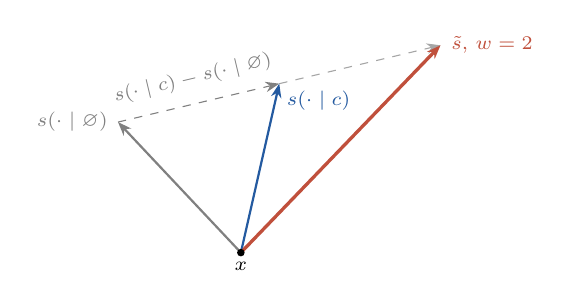
\begin{tikzpicture}[scale=1.95, >={Stealth[length=5pt]}]
\coordinate (O) at (0,0);
\coordinate (U) at (-0.80,0.85);   % unconditional score
\coordinate (C) at (0.25,1.10);    % conditional score
\coordinate (G) at (1.30,1.35);    % guided, w=2: U + 2(C-U)
\draw[->, dashed, gray] (U) -- (C)
  node[midway, above=2pt, sloped, font=\scriptsize]
  {$\score(\cdot \mid c) - \score(\cdot \mid \varnothing)$};
\draw[->, dashed, gray!70] (C) -- (G);
\draw[->, gray, thick] (O) -- (U)
  node[left, font=\scriptsize] {$\score(\cdot \mid \varnothing)$};
\draw[->, cdata, thick] (O) -- (C)
  node[below right=-1pt, font=\scriptsize] {$\score(\cdot \mid c)$};
\draw[->, cnoise, very thick] (O) -- (G)
  node[right, font=\scriptsize] {$\tilde\score$, $w = 2$};
\fill (O) circle (0.7pt) node[below, font=\scriptsize] {$x$};
\end{tikzpicture}
\end{minipage}\hfill
\begin{minipage}[c]{0.57\textwidth}
\centering
\begin{tikzpicture}
\begin{axis}[
  dfm, width=8.4cm, height=5.6cm, axis lines=left,
  xmin=-2.4, xmax=2.4, ymin=0, ymax=2.45,
  xlabel={$x$}, ytick=\empty,
  legend pos=north west, legend cell align=left,
]
\addplot[draw=gray!60, fill=gray!14] table[x=x, y=p] {dfm_figs/guide.dat}
  \closedcycle;
\addlegendentry{$q(x)$}
\addplot[black!60, densely dashed] table[x=x, y=lik] {dfm_figs/guide.dat};
\addlegendentry{$q(c \mid x)$}
\addplot[cdata, thick] table[x=x, y=w1] {dfm_figs/guide.dat};
\addlegendentry{tilted, $w = 1$ (Bayes)}
\addplot[cnoise, thick] table[x=x, y=w3] {dfm_figs/guide.dat};
\addlegendentry{tilted, $w = 3$}
\end{axis}
\end{tikzpicture}
\end{minipage}
\caption{Guidance as score arithmetic. Left: equation \eqref{eq:cfg} at a
single point --- the guided score $\tilde\score$ continues past the
conditional score along the line from unconditional to conditional;
$w = 1$ would stop at $\score(\cdot \mid c)$, $w > 1$ extrapolates.
Right: what the corresponding tilt $q(x)\, q(c \mid x)^w$ (normalized)
does to a bimodal density with a soft classifier for the right-hand class.
At $w = 1$ this is exact Bayesian conditioning: the wrong mode is
suppressed but survives where the classifier is unsure. At $w = 3$ the
surviving mode sharpens and shifts \emph{into} the classifier-confident
region --- prompt adherence up, diversity down, and the mode is no longer
quite where the data was. Now recall the fine print: the sampler applies
this tilt at \emph{every} noise level, which is not the same as diffusing
the tilted data distribution.}
\label{fig:guidance}
\end{figure}

\section{The whole subject on one page}

\begin{center}
\small
\begin{tabular}{@{}p{3.0cm}p{5.3cm}p{5.6cm}@{}}
\toprule
Choice & Options & Comment \\
\midrule
Path of marginals & VP / VE / linear / cosine schedule $(\alpha_t,\sigma_t)$ & a design input, not a discovery; all give Gaussian conditionals \\
Learned wardrobe & $\hat\veps$ / $\hat x_0$ / $\score$ / $\hat v$ & one function, four parameterizations; convert by \eqref{eq:wardrobes} \\
Training identity & DSM \eqref{eq:dsm} or CFM \eqref{eq:cfm} & both use Lemma~\ref{lem:proj}; for Gaussian interpolants, different target dress for the same marginal field \\
Sampler & PF-ODE $\leftrightarrow$ reverse SDE (+ churn) & ODE = fast, reproducible; SDE = self-correcting; a dial \\
Likelihood & $\frac{\dd}{\dd t}\log p = -\nabla\!\cdot\!v$ along the ODE & diffusion inherits CNF's flow-likelihood machinery (\S\ref{sec:likelihood}) \\
Step count & solver order \& step placement (\S\ref{sec:solvers}), curvature, reflow, distillation & the cost model: pay per network call; straightness is wealth \\
Steering & guidance arithmetic \eqref{eq:cfg} & approximate tilting; the $w$ knob trades diversity for adherence \\
\bottomrule
\end{tabular}
\end{center}

\medskip
Two sentences to carry away. \emph{A generative model is a path of distributions from data to
noise plus a velocity that transports it; both the path and the
stochasticity of its traversal are design choices.} \emph{The path's
conditional structure hands you closed-form per-sample regression targets,
and one lemma --- conditional expectation minimizes $L^2$ --- guarantees
that regressing on them learns the true score/velocity: that lemma,
used twice, is the entire trainability of the field.}

\medskip
Operationally, almost every training loop in these notes is the same
five-line program:
\begin{enumerate}
\item sample $x_0 \sim p_{\mathrm{data}}$, $\veps \sim \mathcal{N}(0,I)$,
and $t$;
\item form $x_t = \alpha_t x_0 + \sigma_t \veps$;
\item choose the wardrobe: predict $\veps$, $\score$, $x_0$, or $v$;
\item regress on the corresponding closed-form target with MSE;
\item at sampling time, draw $x_1$ from the noise prior and integrate the
learned ODE or SDE backwards to $t=0$.
\end{enumerate}

\subsection*{Problems}

\begin{enumerate}
\item Prove Tweedie \eqref{eq:tweedie} as outlined in Exercise~1 (if you
have not already), then derive the
$\E[\veps \mid x_t]$ version and confirm the wardrobe conversions
\eqref{eq:wardrobes} are mutually consistent.
\item \label{prob:continuity} Show that \eqref{eq:marg-vel} satisfies the
continuity equation \eqref{eq:continuity} for $q_t$: write
$q_t(x) = \E_{x_0,\veps}\,\delta(x - \alpha_t x_0 - \sigma_t\veps)$,
differentiate in $t$, and integrate by parts. (Read the $\delta$ as the
$w \to 0$ limit of $\mathcal{N}(0, w^2 I)$ densities; or sidestep it by
integrating everything against a smooth test function first, in which
case you are running the Exercise-after-\eqref{eq:fp-general} argument
in reverse.)
\item \label{prob:posterior} Derive the DDPM forward posterior
$q(x_s \mid x_t, x_0)$ for $s < t$ (Gaussian; find its mean and variance),
and verify that the KL terms of \eqref{eq:elbo} reduce to weighted
$\veps$-prediction MSEs.
\item \label{prob:anderson} Anderson by hand. One Euler--Maruyama step
of the forward SDE \eqref{eq:forward-sde} is a Gaussian kernel
$q(x_{t+h} \mid x_t)$. Apply Bayes,
$q(x_t \mid x_{t+h}) \propto q(x_{t+h} \mid x_t)\, q_t(x_t)$, expand
$\log q_t(x_t) \approx \log q_t(x_{t+h}) + (x_t - x_{t+h}) \cdot
\nabla \log q_t(x_{t+h})$, and complete the square. Show the reverse
kernel is Gaussian with mean
$x_{t+h} - h\big[ f_t\, x_{t+h} - g_t^2 \nabla\log q_t(x_{t+h}) \big] + O(h^2)$ and
covariance $g_t^2 h\, I$ --- the reverse SDE \eqref{eq:reverse-sde},
derived in four lines with no stochastic analysis. Where did the factor
of \emph{two} relative to the probability-flow correction come from?
\item Gaussian sandbox, continued: verify the closed forms
\eqref{eq:gauss-score}--\eqref{eq:gauss-vel} asserted in Section~2
(complete the square; check the velocity lands in both wardrobes). Show
that with the linear
schedule the marginal ODE trajectories are straight only if the data is a
single Gaussian and the coupling is the model's own --- then exhibit a
two-component mixture whose marginal trajectories visibly curve.
\item Gaussian sandbox, part II (solvers). For the single-Gaussian data
of the previous problem the probability-flow ODE is linear with a known
solution. Implement Euler, Heun, and DDIM \eqref{eq:ddim} with both
uniform-$t$ and uniform log-SNR grids; measure endpoint error against
the exact flow and reproduce the qualitative content of
Figure~\ref{fig:solvers}. Verify numerically that DDIM becomes exact as
$s \to 0$ (Exercise~\ref{ex:ddim-exact}). Then add the divergence as an
extra integrated state, as in \eqref{eq:likelihood}, and check the
recovered $\log p_0$ against the closed-form Gaussian log-density ---
first with the exact divergence, then with Hutchinson's estimator.
\item Show that one CFG step \eqref{eq:cfg} corresponds to the score of
the unnormalized density $q_t(x)\,\big[q_t(x \mid c)/q_t(x)\big]^w$, and
explain in two sentences why doing this at every $t$ does not sample the
$t = 0$ tilted distribution exactly.
\item (Open-ended.) Implement CFM with the linear schedule on
two-moons in 2D ($\sim$60 lines --- the snippets in Sections~2.2
and~\ref{sec:pfode} are most of them). Plot the learned velocity field at
several $t$, sample with 1, 4, and 50 Euler steps, then do one round of
reflow and repeat. Watch the trajectories straighten. Finally,
implement the \emph{learning-free} competitor: the closed-form
empirical score of the mixture \eqref{eq:qt} over your training points,
plugged into the same ODE. Watch it return the training set, then
reread the ``what training buys'' paragraph of Section~2.2.
\end{enumerate}

\begin{thebibliography}{99}\small
\bibitem{sohl} J.~Sohl-Dickstein et al., ``Deep unsupervised learning
using nonequilibrium thermodynamics,'' ICML 2015. (The origin; reads
remarkably well in hindsight.)
\bibitem{ho} J.~Ho, A.~Jain, P.~Abbeel, ``Denoising diffusion
probabilistic models,'' NeurIPS 2020.
\bibitem{song} Y.~Song et al., ``Score-based generative modeling through
stochastic differential equations,'' ICLR 2021. (The unifying SDE/ODE
paper; source of Section~\ref{sec:pfode}.)
\bibitem{vincent} P.~Vincent, ``A connection between score matching and
denoising autoencoders,'' Neural Computation 2011. (Lemma~\ref{lem:proj},
instance 1.)
\bibitem{lipman} Y.~Lipman et al., ``Flow matching for generative
modeling,'' ICLR 2023. (Lemma~\ref{lem:proj}, instance 2.)
\bibitem{liu} X.~Liu, C.~Gong, Q.~Liu, ``Flow straight and fast: learning
to generate and transfer data with rectified flow,'' ICLR 2023.
\bibitem{albergo} M.~Albergo, N.~Boffi, E.~Vanden-Eijnden, ``Stochastic
interpolants,'' 2023. (The general framework containing all the schedules.)
\bibitem{karras} T.~Karras et al., ``Elucidating the design space of
diffusion-based generative models,'' NeurIPS 2022. (The engineering
companion: schedules, parameterizations, samplers, ablated.)
\bibitem{anderson} B.~D.~O.~Anderson, ``Reverse-time diffusion equation
models,'' Stochastic Processes and their Applications, 1982.
\bibitem{ddim} J.~Song, C.~Meng, S.~Ermon, ``Denoising diffusion
implicit models,'' ICLR 2021. (The update \eqref{eq:ddim}, derived there
very differently.)
\bibitem{dpmsolver} C.~Lu et al., ``DPM-Solver: a fast ODE solver for
diffusion probabilistic model sampling in around 10 steps,'' NeurIPS
2022. (Higher-order solvers in the coordinates of
Section~\ref{sec:ddim}.)
\bibitem{ffjord} W.~Grathwohl et al., ``FFJORD: free-form continuous
dynamics for scalable reversible generative models,'' ICLR 2019.
(Hutchinson-traced likelihoods, Section~\ref{sec:likelihood}.)
\bibitem{bb} J.-D.~Benamou, Y.~Brenier, ``A computational fluid
mechanics solution to the Monge--Kantorovich mass transfer problem,''
Numerische Mathematik, 2000. (The kinetic-energy formulation
\eqref{eq:bb} of optimal transport.)
\bibitem{sarkka} S.~S\"arkk\"a, A.~Solin, ``Applied stochastic
differential equations,'' Cambridge University Press, 2019. (Everything
in Section~\ref{sec:sde}, at textbook pace and with the analysis done
honestly.)
\bibitem{hairer} E.~Hairer, S.~P.~N\o rsett, G.~Wanner, ``Solving
ordinary differential equations I: nonstiff problems,'' Springer, 1993.
(The solver's-eye view, fully grown.)
\end{thebibliography}

\end{document}
